\chapter{Dasar Dasar Code OpenCV}
\section{Menampilkan gambar}
\subsection{Menampilkan Gambar}

\lstinputlisting{src/cv2.py}
\begin{enumerate}
	\item lakukan Import library open cv yaitu cv2
	\item kemudian panggil file foto menggunakan kode seperti di atas, membuat terlebihdahulu variabel img, kemudian cv2.imread nama file dan nomor untuk gradiasi warnanya, pada bagian ini menggunakan angka 1 yang artinya mengikuti foto aslinya.
	\item lakukan print untuk menampilkan gambar
	\item kemudian buat frame untuk menampilkan gambar menggunakan imshow dengan nama frame image.
	\item kemudian gunakan waitKey untuk membuat frame agar tidak langsung mati atau tertutup otomatis.
	\item destroyAllWindows digunakan untuk menutup frame.
\end{enumerate}

\begin{figure}[ht]
\centering
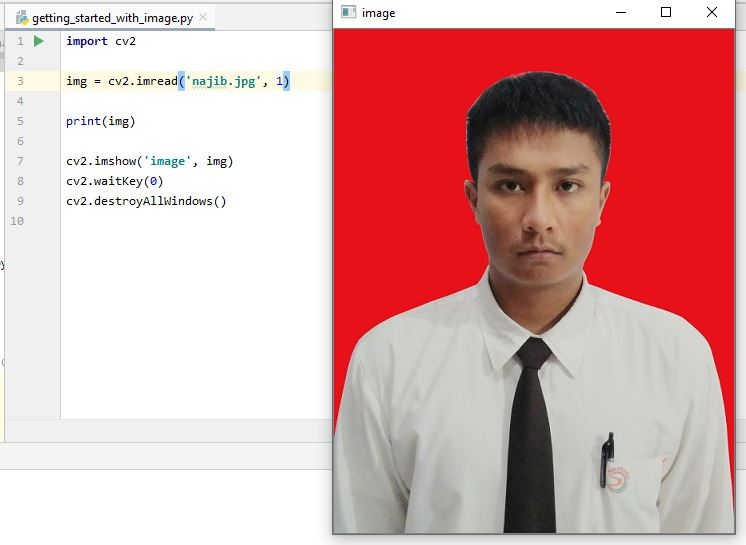
\includegraphics[scale=0.5]{figures/2,2.jpg}
\caption{Menampilkan gambar}
\label{contoh}
\end{figure}
Hasil yang ditampilkan sama seperti foto aslinya karna tidak ada dari foto yang di rubah sama sekali, kodingan ini hanya bertujuan untuk menampilkan gambar saja.

\newpage
\subsection{Menampilkan Gambar dan merubah kontras warnanya}
\lstinputlisting{src/cv1.py}
\begin{enumerate}
	\item lakukan Import library open cv yaitu cv2
	\item kemudian panggil file foto menggunakan kode seperti di atas, membuat terlebihdahulu variabel img, kemudian cv2.imread nama file dan nomor untuk gradiasi warnanya, pada bagian ini menggunakan angka 0 merubah gambar menjadi hitam putih.
	\item lakukan print untuk menampilkan gambar
	\item kemudian buat frame untuk menampilkan gambar menggunakan imshow dengan nama frame image.
	\item kemudian gunakan waitKey untuk membuat frame agar tidak langsung mati atau tertutup otomatis.
	\item destroyAllWindows digunakan untuk menutup frame.
\end{enumerate}


\newpage
\begin{figure}[ht]
\centering
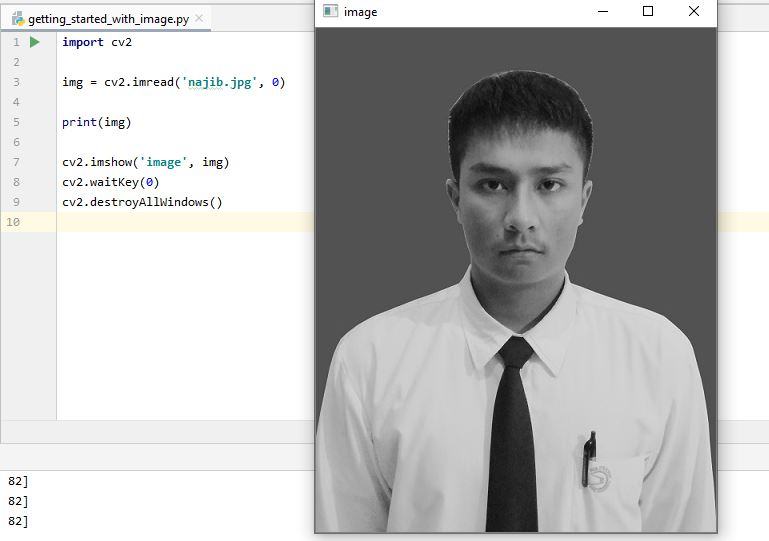
\includegraphics[scale=0.6]{figures/2,1.jpg}
\caption{Merubah kontras warna}
\label{contoh}
\end{figure}

Pada bagian kodingan ini foto di rubah kontras warnanya menjadi hitam putih, pada kodingan sebelumnya yang di rubah hanya satu huruf saja untu menjadikan foto ini menjadi seperti ini. yaitu pada bagian imread nya menjadi 0.

\newpage
\subsection{Menyimpan Gambar menggunakan kode opencv}
\lstinputlisting{src/cv3.py}
\begin{enumerate}
	\item lakukan Import library open cv yaitu cv2
	\item kemudian panggil file foto menggunakan kode seperti di atas, membuat terlebihdahulu variabel img, kemudian cv2.imread nama file dan nomor untuk gradiasi warnanya, pada bagian ini menggunakan angka 0 merubah gambar menjadi hitam putih.
	\item lakukan print untuk menampilkan gambar
	\item kemudian buat frame untuk menampilkan gambar menggunakan imshow dengan nama frame image.
	\item kemudian gunakan waitKey untuk membuat frame agar tidak langsung mati atau tertutup otomatis.
	\item destroyAllWindows digunakan untuk menutup frame.
	\item terakhir gambar disimpan menggunakan kode imwrite, pertama tuliskan nama gambar yang akan disimpan beserta formatgambarnya, kemudian kode img untuk menyatakan yang disimpan tersebut adalah gambar.
\end{enumerate}

\newpage
\begin{figure}[ht]
\centering
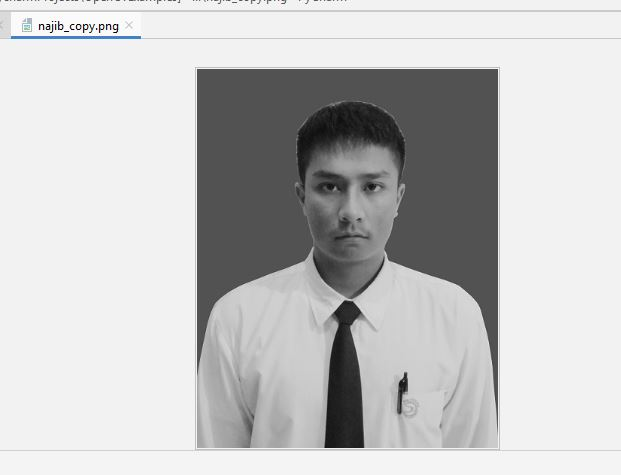
\includegraphics[scale=0.7]{figures/2,3.jpg}
\caption{Menyimpan gambar}
\label{contoh}
\end{figure}

Gambar berhasil disimpan dengan nama najibcopy.png, gambar disimpan sesuai yang telah di edit kontras warnanya menjadi hitam putih sesuai cede yang kita jalankan.

\newpage
\section{Menjalankan kamera leptop}
\subsection{Menjalankan video kamera leptop}
\lstinputlisting{src/cv4.py}
\begin{enumerate}
	\item lakukan Import library open cv yaitu cv2
	\item kemudian buat variable baru dengan nama cap kemudian panggil VideoCapture(0) yang artinya menjalankan kamera leptop.
	\item membuat while yaitu perulangan membuka frame
	\item kemudian didalam perulangan tersebut terdapat frame yang membaca atau merekam video.
	\item kemudian buat frame dengan nama frame
	\item kemudian gunakan waitKey untuk membuat frame agar tidak langsung mati atau tertutup otomatis.
	\item release untuk menutup videocapture
	\item destroyAllWindows digunakan untuk menutup frame.
\end{enumerate}

\newpage
\begin{figure}[ht]
\centering
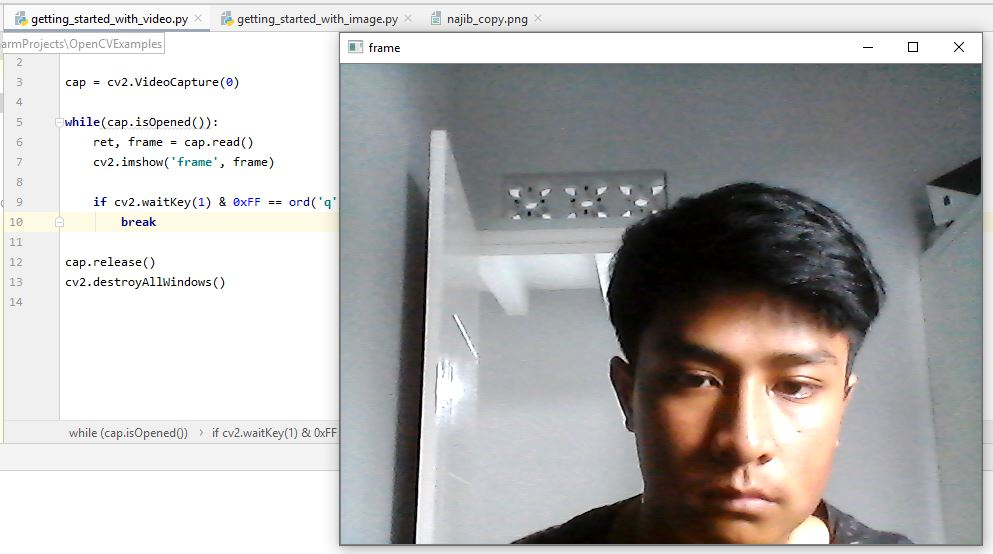
\includegraphics[scale=0.5]{figures/2,4.jpg}
\caption{Menggunakan kamera leptop}
\label{contoh}
\end{figure}

Pada videocpture ini hanya merekam menggunakan kamera leptop saja belum masuk ke pengolahan gambar.

\newpage
\subsection{Merubah kontras warna pada video}
\lstinputlisting{src/cv5.py}
\begin{enumerate}
	\item lakukan Import library open cv yaitu cv2
	\item kemudian buat variable baru dengan nama cap kemudian panggil VideoCapture(0) yang artinya menjalankan kamera leptop.
	\item membuat while yaitu perulangan membuka frame
	\item kemudian didalam perulangan tersebut terdapat frame yang membaca atau merekam video.
	\item buat variable dengan nama gray karna kita mau berubah kontras warnanya menjadi hitam putih, kemudian panggil cvtColor didalam frame dengan warna abu abu.
	\item kemudian buat frame dengan nama frame
	\item kemudian gunakan waitKey untuk membuat frame agar tidak langsung mati atau tertutup otomatis.
	\item release untuk menutup videocapture
	\item destroyAllWindows digunakan untuk menutup frame.
\end{enumerate}

\newpage
\begin{figure}[ht]
\centering
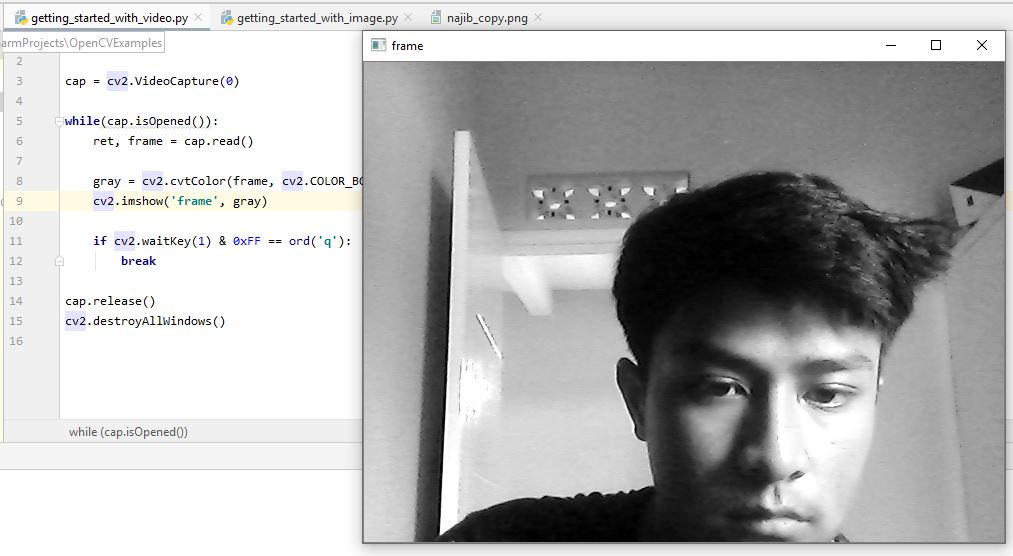
\includegraphics[scale=0.45]{figures/2,5.jpg}
\caption{Kontras warna video}
\label{contoh}
\end{figure}

Pada videocpture ini video sudah di rubah kontras warnanya menjadi abu abu, kita bisa rubah sesuai yang kita inginkan.

\newpage
\subsection{Mengetahui ukuran frame yang ditampilkan}
\lstinputlisting{src/cv6.py}
\begin{enumerate}
	\item lakukan Import library open cv yaitu cv2
	\item kemudian buat variable baru dengan nama cap kemudian panggil VideoCapture(0) yang artinya menjalankan kamera leptop.
	\item membuat while yaitu perulangan membuka frame
	\item kemudian didalam perulangan tersebut terdapat frame yang membaca atau merekam video.
	\item kita cukup print mengambil dari videocapture dan panggil CAP PROP FRAME WIDTH untuk mengetahui ukuran lebarnya dan CAP PROP FRAME HEIGHT untuk ukuran tingginya 
	\item buat variable dengan nama gray karna kita mau berubah kontras warnanya menjadi hitam putih, kemudian panggil cvtColor didalam frame dengan warna abu abu.
	\item kemudian buat frame dengan nama frame
	\item kemudian gunakan waitKey untuk membuat frame agar tidak langsung mati atau tertutup otomatis.
	\item release untuk menutup videocapture
	\item destroyAllWindows digunakan untuk menutup frame.
\end{enumerate}

\newpage
\begin{figure}[ht]
\centering
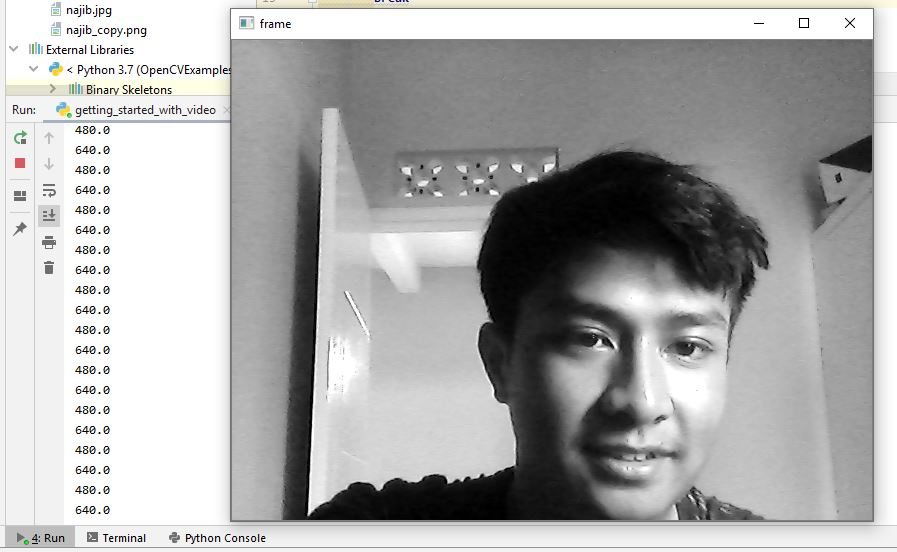
\includegraphics[scale=0.52]{figures/2,6.jpg}
\caption{Ukuran Frame video}
\label{contoh}
\end{figure}

Maka akan ditampilkan secara berulang karna berada pada while dan pada bagian videocapture juga jika tidak di lakukan perulangan maka sekali muncul akan langsung keluar secara otomatis.

\newpage
\subsection{Menyimpan video}
\lstinputlisting{src/cv7.py}
\begin{enumerate}
	\item lakukan Import library open cv yaitu cv2
	\item kemudian buat variable baru dengan nama cap kemudian panggil VideoCapture(0) yang artinya menjalankan kamera leptop.
	\item membuat variabel fourcc untuk merekam video yang dijalankan.
	\item membuat variable out untuk menyimpan video dengan nama najib.avi dan frame berukuran 640,480.
	\item melakukan print apakah true atau false kamera leptop terbuka.
	\item membuat while yaitu perulangan membuka frame
	\item kemudian didalam perulangan tersebut terdapat frame yang membaca atau merekam video.
	\item jika kamera true merekam maka akan melakukan perintah.
	\item kita cukup print mengambil dari videocapture dan panggil CAP PROP FRAME WIDTH untuk mengetahui ukuran lebarnya dan 
	\item kita cukup print mengambil dari videocapture dan panggil CAP PROP FRAME HEIGHT untuk ukuran tingginya 
	\item buat variable dengan nama gray karna kita mau berubah kontras warnanya menjadi hitam putih, kemudian panggil cvtColor didalam frame dengan warna abu abu.
	\item kemudian buat frame dengan nama frame
	\item kemudian gunakan waitKey untuk membuat frame agar tidak langsung mati atau tertutup otomatis.
	\item release untuk menutup videocapture
	\item destroyAllWindows digunakan untuk menutup frame.
\end{enumerate}

\begin{figure}[ht]
\centering
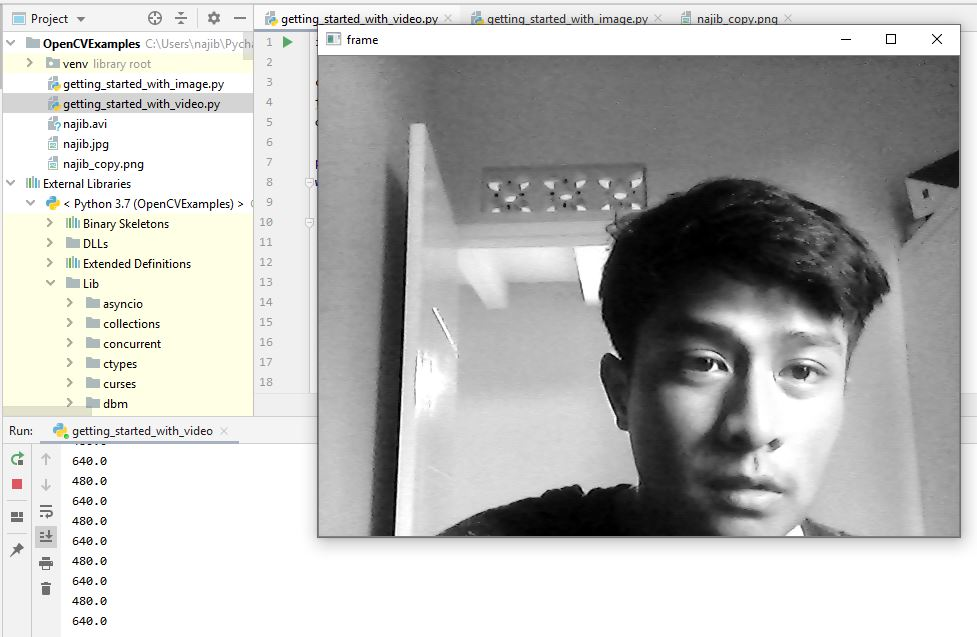
\includegraphics[scale=0.5]{figures/2,7.jpg}
\caption{Setelah dijalankan file tersimpan}
\label{contoh}
\end{figure}

\newpage
\begin{figure}[ht]
\centering
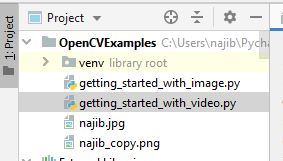
\includegraphics[scale=0.8]{figures/2,7,1.jpg}
\caption{File Sebelum dijalankan}
\label{contoh}
\end{figure}

\begin{figure}[ht]
\centering
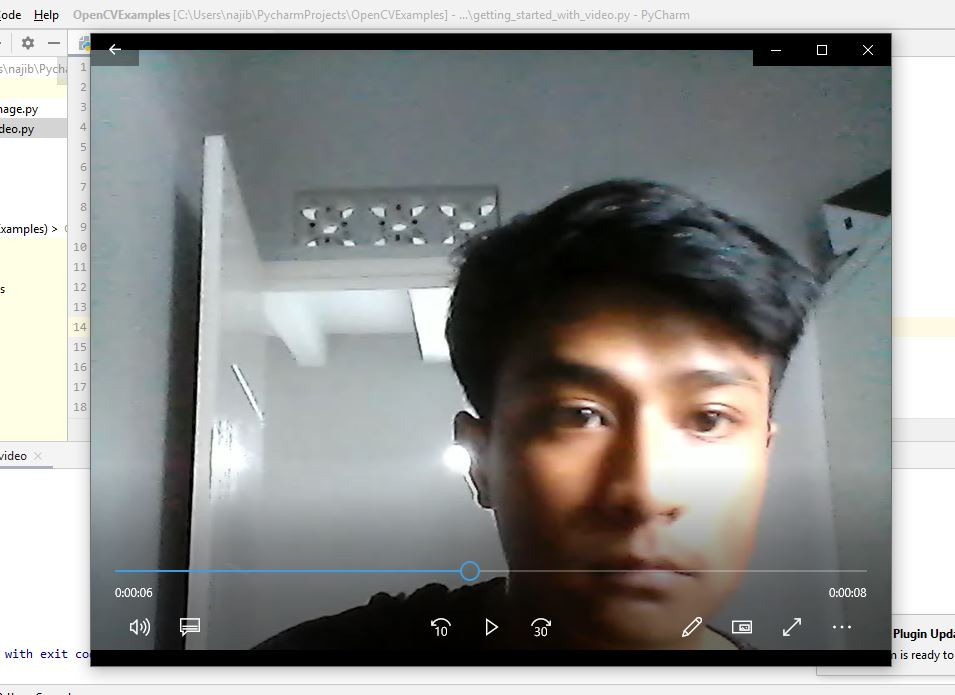
\includegraphics[scale=0.5]{figures/2,7,2.jpg}
\caption{Video yang sudah di simpan}
\label{contoh}
\end{figure}

Video tersimpan langsung ke folder yang dituju, video dapat disesuaikan formatnya sesuai yang kita mau.

\newpage
\section{Menggambar Geometric Pada Foto}
\subsection{Membuat garis}
\lstinputlisting{src/cv8.py}
\begin{enumerate}
	\item lakukan Import library open cv yaitu cv2
	\item kemudian panggil file foto menggunakan kode seperti di atas, membuat terlebihdahulu variabel img, kemudian cv2.imread nama file dan nomor untuk gradiasi warnanya, pada bagian ini menggunakan angka 0 yang artinya gambar berubah menjadi hitam putih.
	\item kemudian buat garis menggunakan cv2.line, 0,0 merupakan dimana titik awal garis tersebut dan 255,255 merupakan titik akhir dari garis tersebut, kemudian selanjutnya adahal warna dari garis tersebut, dan yang terakhir adalah ketebalan dari garis yang dibuat.
	\item kemudian buat frame untuk menampilkan gambar menggunakan imshow dengan nama frame image.
	\item kemudian gunakan waitKey untuk membuat frame agar tidak langsung mati atau tertutup otomatis.
	\item destroyAllWindows digunakan untuk menutup frame.
\end{enumerate}

\newpage
\begin{figure}[ht]
\centering
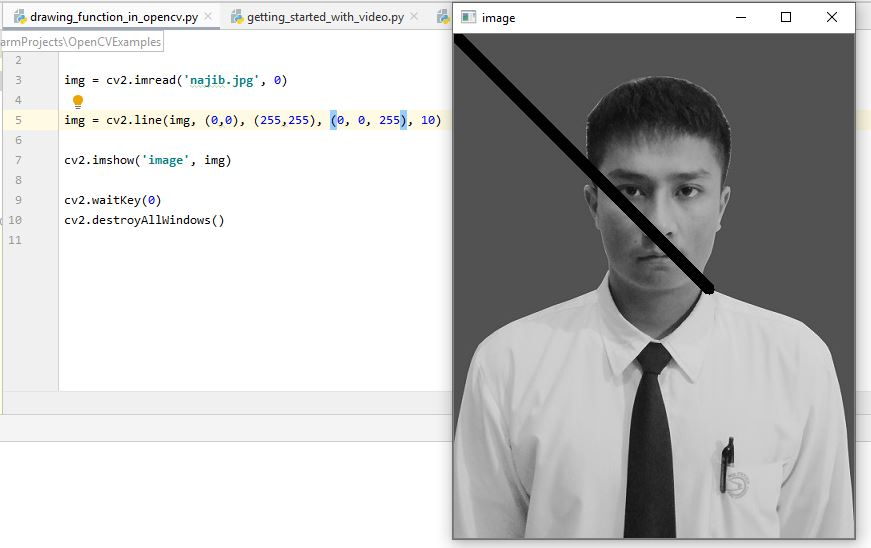
\includegraphics[scale=0.55]{figures/2,8.jpg}
\caption{MMembuat garis}
\label{contoh}
\end{figure}

garis bisa kita taruh dimana saja sesuai yang diinginkan kenapa garisnya menjulur dari pojok kiri atas ke tengah karna titik 0,0 berada di pojok kiri atas sedangkan titik 255,255 berada di tengah tengah gambar, gambar ini pun menjadi hitam putih karna di awal pada imread nya diberikan angka 0 yang membuat gambar berubah menjadi hitam putih.

\newpage
\subsection{Membuat warna warna pada garis}
\lstinputlisting{src/cv9.py}
\begin{enumerate}
	\item lakukan Import library open cv yaitu cv2
	\item kemudian panggil file foto menggunakan kode seperti di atas, membuat terlebihdahulu variabel img, kemudian cv2.imread nama file dan nomor untuk gradiasi warnanya, pada bagian ini menggunakan angka 1 yang artinya mengikuti foto aslinya.
	\item kemudian buat garis menggunakan cv2.line, 0,0 merupakan dimana titik awal garis tersebut dan 255,255 merupakan titik akhir dari garis tersebut, kemudian selanjutnya adalah warna dari garis tersebut, dan yang terakhir adalah ketebalan dari garis yang dibuat.
	\item kemudian buat frame untuk menampilkan gambar menggunakan imshow dengan nama frame image.
	\item kemudian gunakan waitKey untuk membuat frame agar tidak langsung mati atau tertutup otomatis.
	\item destroyAllWindows digunakan untuk menutup frame.
\end{enumerate}

\newpage
\begin{figure}[ht]
\centering
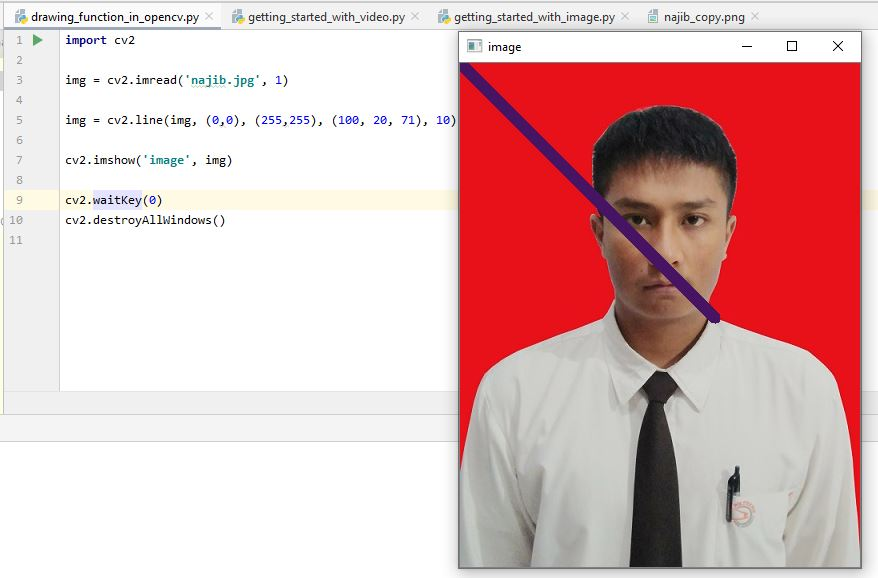
\includegraphics[scale=0.55]{figures/2,9.jpg}
\caption{Membuat garis}
\label{contoh}
\end{figure}

garis bisa kita taruh dimana saja sesuai yang diinginkan kenapa garisnya menjulur dari pojok kiri atas ke tengah karna titik 0,0 berada di pojok kiri atas sedangkan titik 255,255 berada di tengah tengah gambar, gambar menjadi seperti aslinya karna pada imreadnya 1.

\newpage
\begin{figure}[ht]
\centering
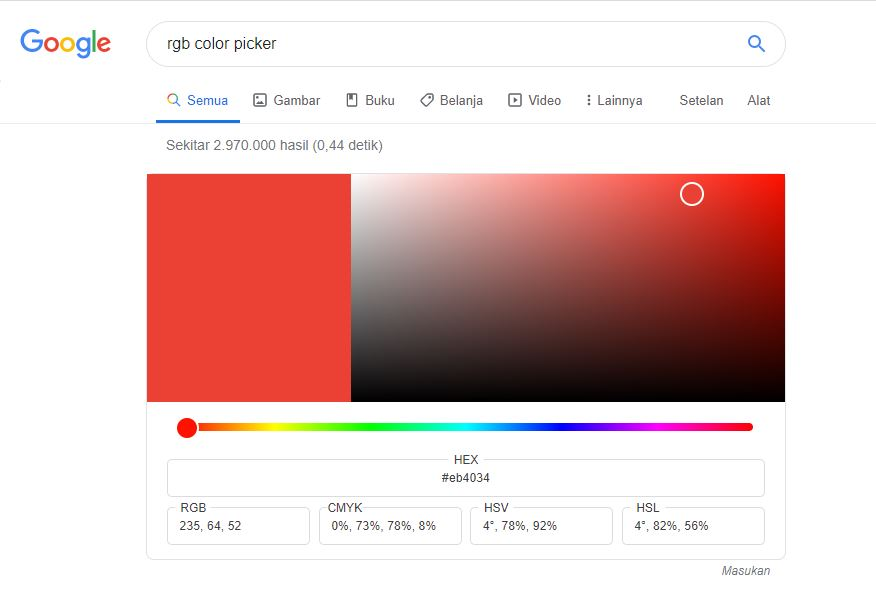
\includegraphics[scale=0.55]{figures/2,9,1.jpg}
\caption{Nomor Nomor warna}
\label{contoh}
\end{figure}

jika kita ingin warna yang sesuai dengan keinginan kita, kita bisa langsung search di google seperti pada gambar maka akan ada nomor nomornya untuk setiap warna.

\newpage
\subsection{Membuat garis panah}
\lstinputlisting{src/cv10.py}
\begin{enumerate}
	\item lakukan Import library open cv yaitu cv2
	\item kemudian panggil file foto menggunakan kode seperti di atas, membuat terlebihdahulu variabel img, kemudian cv2.imread nama file dan nomor untuk gradiasi warnanya, pada bagian ini menggunakan angka 1 yang artinya mengikuti foto aslinya.
	\item kemudian buat garis menggunakan cv2.line, 0,0 merupakan dimana titik awal garis tersebut dan 255,255 merupakan titik akhir dari garis tersebut, kemudian selanjutnya adalah warna dari garis tersebut, dan yang terakhir adalah ketebalan dari garis yang dibuat.
	\item kemudian buat garis panah menggunakan cv2.arrowedLine, 0,0 merupakan dimana titik awal garis tersebut dan 255,255 merupakan titik akhir dari garis tersebut, kemudian selanjutnya adalah warna dari garis tersebut, dan yang terakhir adalah ketebalan dari garis yang dibuat.
	\item kemudian buat frame untuk menampilkan gambar menggunakan imshow dengan nama frame image.
	\item kemudian gunakan waitKey untuk membuat frame agar tidak langsung mati atau tertutup otomatis.
	\item destroyAllWindows digunakan untuk menutup frame.
\end{enumerate}

\newpage
\begin{figure}[ht]
\centering
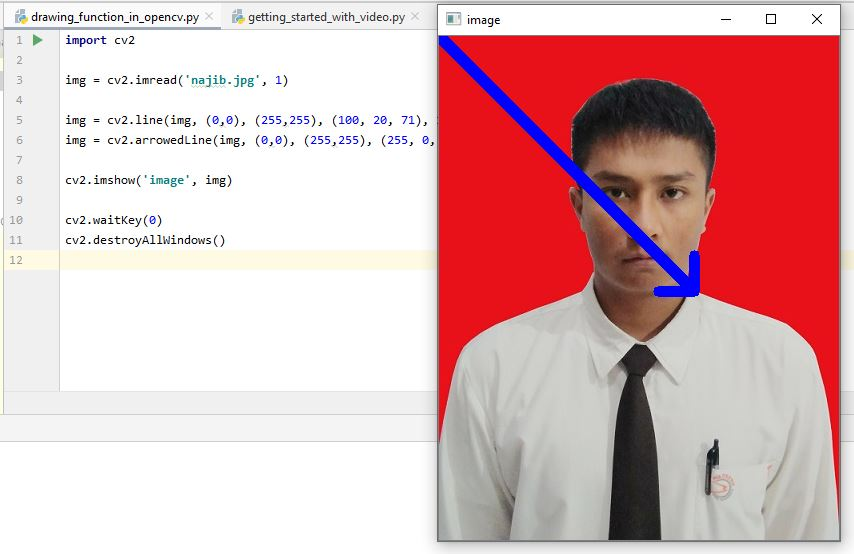
\includegraphics[scale=0.55]{figures/2,10.jpg}
\caption{Membuat garis panah}
\label{contoh}
\end{figure}

Garis panah yang dibuat menumpuk dengan garis yang awal jadi yang di lihat seperti garis yang sebelumnya hilang padahal garis tersebut tertumpuk.

\newpage
\subsection{Membuat garis kotak}
\lstinputlisting{src/cv11.py}
\begin{enumerate}
	\item lakukan Import library open cv yaitu cv2
	\item kemudian panggil file foto menggunakan kode seperti di atas, membuat terlebihdahulu variabel img, kemudian cv2.imread nama file dan nomor untuk gradiasi warnanya, pada bagian ini menggunakan angka 1 yang artinya mengikuti foto aslinya.
	\item kemudian buat garis menggunakan cv2.line, 0,0 merupakan dimana titik awal garis tersebut dan 255,255 merupakan titik akhir dari garis tersebut, kemudian selanjutnya adalah warna dari garis tersebut, dan yang terakhir adalah ketebalan dari garis yang dibuat.
	\item kemudian buat garis panah menggunakan cv2.arrowedLine, 0,0 merupakan dimana titik awal garis tersebut dan 255,255 merupakan titik akhir dari garis tersebut, kemudian selanjutnya adalah warna dari garis tersebut, dan yang terakhir adalah ketebalan dari garis yang dibuat.
	\item kemudian buat garis kotak menggunakan cv2.rectangle, 384,0 merupakan dimana titik awal garis tersebut dan 210,210 merupakan titik akhir dari garis tersebut, kemudian selanjutnya adalah warna dari garis tersebut, dan yang terakhir adalah ketebalan dari garis yang dibuat.
	\item kemudian buat frame untuk menampilkan gambar menggunakan imshow dengan nama frame image.
	\item kemudian gunakan waitKey untuk membuat frame agar tidak langsung mati atau tertutup otomatis.
	\item destroyAllWindows digunakan untuk menutup frame.
\end{enumerate}

\newpage
\begin{figure}[ht]
\centering
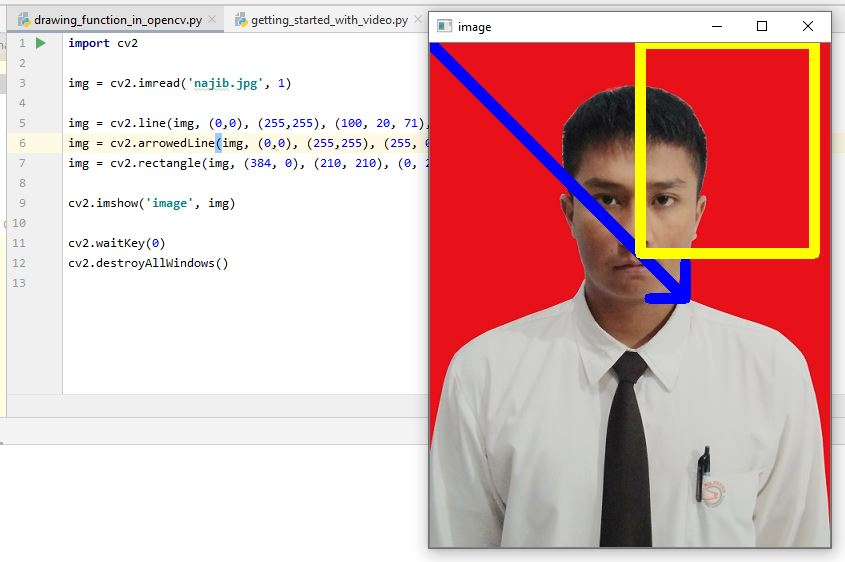
\includegraphics[scale=0.55]{figures/2,11.jpg}
\caption{Membuat garis kotak}
\label{contoh}
\end{figure}

Garis kotak ini bisa kita atur mau warna yang bagaimana, ukuran yang bagaimana, dan posisi yang bagaimana sesuai yang di inginkan dan sesuai kebutuhannya.

\newpage
\subsection{Membuat kotak}
\lstinputlisting{src/cv12.py}
\begin{enumerate}
	\item lakukan Import library open cv yaitu cv2
	\item kemudian panggil file foto menggunakan kode seperti di atas, membuat terlebihdahulu variabel img, kemudian cv2.imread nama file dan nomor untuk gradiasi warnanya, pada bagian ini menggunakan angka 1 yang artinya mengikuti foto aslinya.
	\item kemudian buat garis menggunakan cv2.line, 0,0 merupakan dimana titik awal garis tersebut dan 255,255 merupakan titik akhir dari garis tersebut, kemudian selanjutnya adalah warna dari garis tersebut, dan yang terakhir adalah ketebalan dari garis yang dibuat.
	\item kemudian buat garis panah menggunakan cv2.arrowedLine, 0,0 merupakan dimana titik awal garis tersebut dan 255,255 merupakan titik akhir dari garis tersebut, kemudian selanjutnya adalah warna dari garis tersebut, dan yang terakhir adalah ketebalan dari garis yang dibuat.
	\item kemudian buat garis kotak menggunakan cv2.rectangle, 384,0 merupakan dimana titik awal garis tersebut dan 210,210 merupakan titik akhir dari garis tersebut, kemudian selanjutnya adalah warna dari garis tersebut, dan yang terakhir adalah -1 yang membuat kotak terisi full karna jika plus yang membesar adalah bagian luarnya juka min yang membesar adalah bagian dalamnya jika minus maka akan full.
	\item kemudian buat frame untuk menampilkan gambar menggunakan imshow dengan nama frame image.
	\item kemudian gunakan waitKey untuk membuat frame agar tidak langsung mati atau tertutup otomatis.
	\item destroyAllWindows digunakan untuk menutup frame.
\end{enumerate}

\newpage
\begin{figure}[ht]
\centering
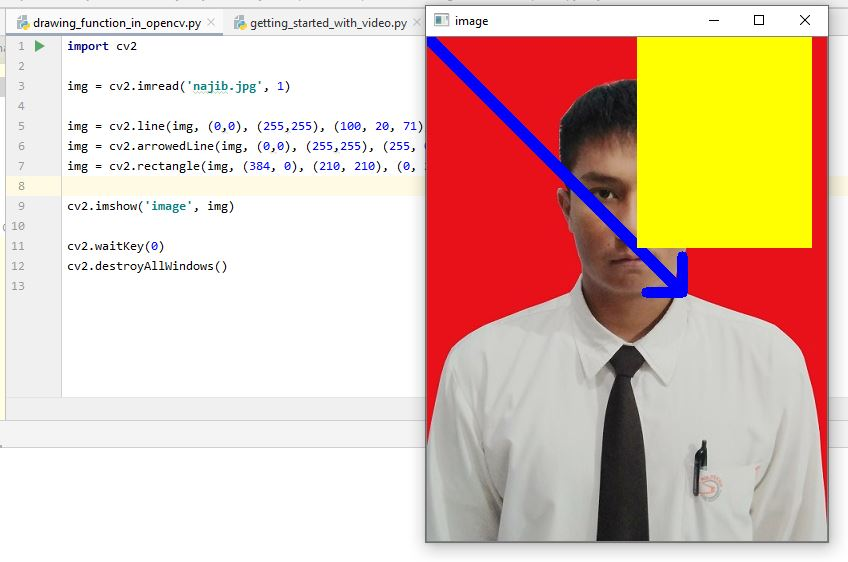
\includegraphics[scale=0.55]{figures/2,12.jpg}
\caption{Membuat kotak}
\label{contoh}
\end{figure}

Garis kotak ini bisa kita atur mau warna yang bagaimana, ukuran yang bagaimana, dan posisi yang bagaimana sesuai yang di inginkan dan sesuai kebutuhannya.

\newpage
\subsection{Membuat garis Lingkaran}
\lstinputlisting{src/cv13.py}
\begin{enumerate}
	\item lakukan Import library open cv yaitu cv2
	\item kemudian panggil file foto menggunakan kode seperti di atas, membuat terlebihdahulu variabel img, kemudian cv2.imread nama file dan nomor untuk gradiasi warnanya, pada bagian ini menggunakan angka 1 yang artinya mengikuti foto aslinya.
	\item kemudian buat garis menggunakan cv2.line, 0,0 merupakan dimana titik awal garis tersebut dan 255,255 merupakan titik akhir dari garis tersebut, kemudian selanjutnya adalah warna dari garis tersebut, dan yang terakhir adalah ketebalan dari garis yang dibuat.
	\item kemudian buat garis panah menggunakan cv2.arrowedLine, 0,0 merupakan dimana titik awal garis tersebut dan 255,255 merupakan titik akhir dari garis tersebut, kemudian selanjutnya adalah warna dari garis tersebut, dan yang terakhir adalah ketebalan dari garis yang dibuat.
	\item kemudian buat garis kotak menggunakan cv2.rectangle, 384,0 merupakan dimana titik awal garis tersebut dan 210,210 merupakan titik akhir dari garis tersebut, kemudian selanjutnya adalah warna dari garis tersebut, dan yang terakhir adalah ketebalan dari garis yang dibuat.
	\item kemudian buat garis kotak menggunakan cv2.circle, 320,63 merupakan dimana titik awal garis tersebut dan 63 merupakan titik tengah, kemudian selanjutnya adalah warna dari garis tersebut, dan yang terakhir adalah -1 yang membuat kotak terisi full karna jika plus yang membesar adalah bagian luarnya juka min yang membesar adalah bagian dalamnya jika minus maka akan full.
	\item kemudian buat frame untuk menampilkan gambar menggunakan imshow dengan nama frame image.
	\item kemudian gunakan waitKey untuk membuat frame agar tidak langsung mati atau tertutup otomatis.
	\item destroyAllWindows digunakan untuk menutup frame.
\end{enumerate}

\begin{figure}[ht]
\centering
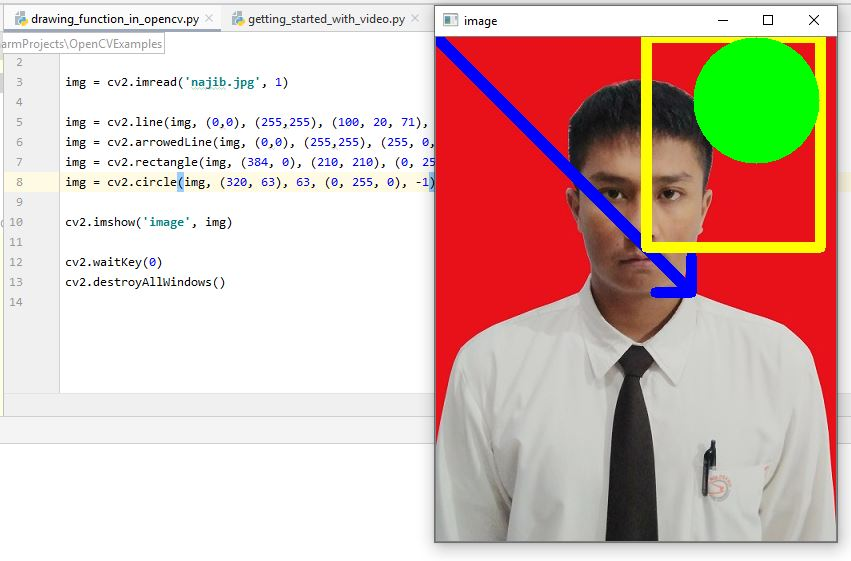
\includegraphics[scale=0.55]{figures/2,13.jpg}
\caption{Membuat garis lingkaran}
\label{contoh}
\end{figure}

Garis Lingkaran ini bisa kita atur mau warna yang bagaimana, ukuran yang bagaimana, dan posisi yang bagaimana sesuai yang di inginkan dan sesuai kebutuhannya.

\newpage
\subsection{Membuat Text}
\lstinputlisting{src/cv14.py}
\begin{enumerate}
	\item lakukan Import library open cv yaitu cv2
	\item kemudian panggil file foto menggunakan kode seperti di atas, membuat terlebihdahulu variabel img, kemudian cv2.imread nama file dan nomor untuk gradiasi warnanya, pada bagian ini menggunakan angka 1 yang artinya mengikuti foto aslinya.
	\item kemudian buat garis menggunakan cv2.line, 0,0 merupakan dimana titik awal garis tersebut dan 255,255 merupakan titik akhir dari garis tersebut, kemudian selanjutnya adalah warna dari garis tersebut, dan yang terakhir adalah ketebalan dari garis yang dibuat.
	\item kemudian buat garis panah menggunakan cv2.arrowedLine, 0,0 merupakan dimana titik awal garis tersebut dan 255,255 merupakan titik akhir dari garis tersebut, kemudian selanjutnya adalah warna dari garis tersebut, dan yang terakhir adalah ketebalan dari garis yang dibuat.
	\item kemudian buat garis kotak menggunakan cv2.rectangle, 384,0 merupakan dimana titik awal garis tersebut dan 210,210 merupakan titik akhir dari garis tersebut, kemudian selanjutnya adalah warna dari garis tersebut, dan yang terakhir adalah ketebalan dari garis yang dibuat.
	\item kemudian buat garis kotak menggunakan cv2.circle, 320,63 merupakan dimana titik awal garis tersebut dan 63 merupakan titik tengah, kemudian selanjutnya adalah warna dari garis tersebut, dan yang terakhir adalah -1 yang membuat kotak terisi full karna jika plus yang membesar adalah bagian luarnya juka min yang membesar adalah bagian dalamnya jika minus maka akan full.
	\item tentukan fontnya terlebih dahulu
	\item kemudian gunakan putText atur sesuai seperti pada gambar.
	\item kemudian buat frame untuk menampilkan gambar menggunakan imshow dengan nama frame image.
	\item kemudian gunakan waitKey untuk membuat frame agar tidak langsung mati atau tertutup otomatis.
	\item destroyAllWindows digunakan untuk menutup frame.
\end{enumerate}

\begin{figure}[ht]
\centering
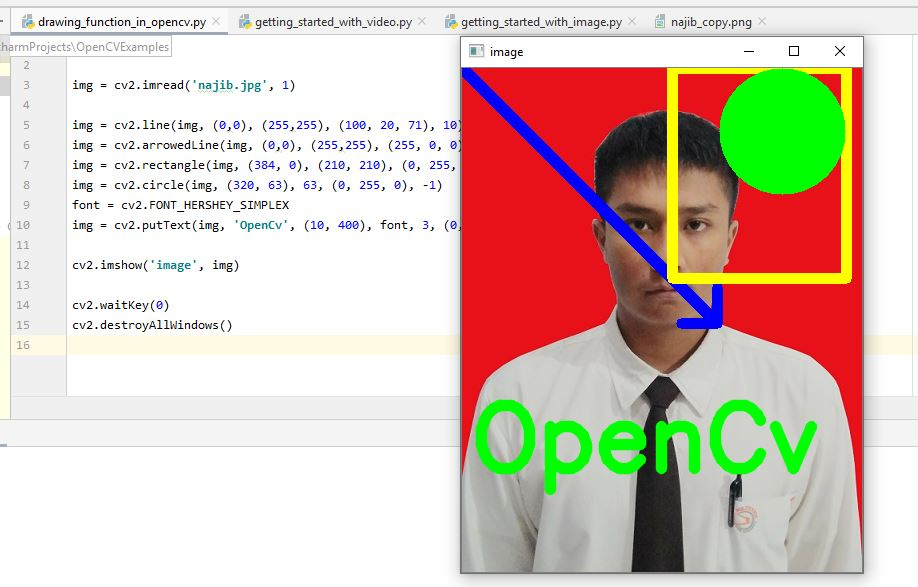
\includegraphics[scale=0.55]{figures/2,14.jpg}
\caption{Membuat Text}
\label{contoh}
\end{figure}

Text ini bisa kita buat sesuai kata kata yang di inginkan dan kata kata yang sesuai pada gambar, mau warna yang bagaimana, ukuran yang bagaimana, dan posisi yang bagaimana sesuai yang di inginkan dan sesuai kebutuhannya.

\newpage
\section{Frame Numpay}
\subsection{Membuat Frame menggunakan Numpay}
\lstinputlisting{src/cv15.py}
\begin{enumerate}
	\item lakukan import numpay as np
	\item lakukan Import library open cv yaitu cv2
	\item kemudian buat frame dari numpy yaitu zeros, kemudian ukuran fram dan warna dari fram, yang di buat adalah hitam.
	\item kemudian buat garis menggunakan cv2.line, 0,0 merupakan dimana titik awal garis tersebut dan 255,255 merupakan titik akhir dari garis tersebut, kemudian selanjutnya adalah warna dari garis tersebut, dan yang terakhir adalah ketebalan dari garis yang dibuat.
	\item kemudian buat garis panah menggunakan cv2.arrowedLine, 0,0 merupakan dimana titik awal garis tersebut dan 255,255 merupakan titik akhir dari garis tersebut, kemudian selanjutnya adalah warna dari garis tersebut, dan yang terakhir adalah ketebalan dari garis yang dibuat.
	\item kemudian buat garis kotak menggunakan cv2.rectangle, 384,0 merupakan dimana titik awal garis tersebut dan 210,210 merupakan titik akhir dari garis tersebut, kemudian selanjutnya adalah warna dari garis tersebut, dan yang terakhir adalah ketebalan dari garis yang dibuat.
	\item kemudian buat garis kotak menggunakan cv2.circle, 320,63 merupakan dimana titik awal garis tersebut dan 63 merupakan titik tengah, kemudian selanjutnya adalah warna dari garis tersebut, dan yang terakhir adalah -1 yang membuat kotak terisi full karna jika plus yang membesar adalah bagian luarnya juka min yang membesar adalah bagian dalamnya jika minus maka akan full.
	\item tentukan fontnya terlebih dahulu
	\item kemudian gunakan putText atur sesuai seperti pada gambar.
	\item kemudian buat frame untuk menampilkan gambar menggunakan imshow dengan nama frame image.
	\item kemudian gunakan waitKey untuk membuat frame agar tidak langsung mati atau tertutup otomatis.
	\item destroyAllWindows digunakan untuk menutup frame.
\end{enumerate}

\begin{figure}[ht]
\centering
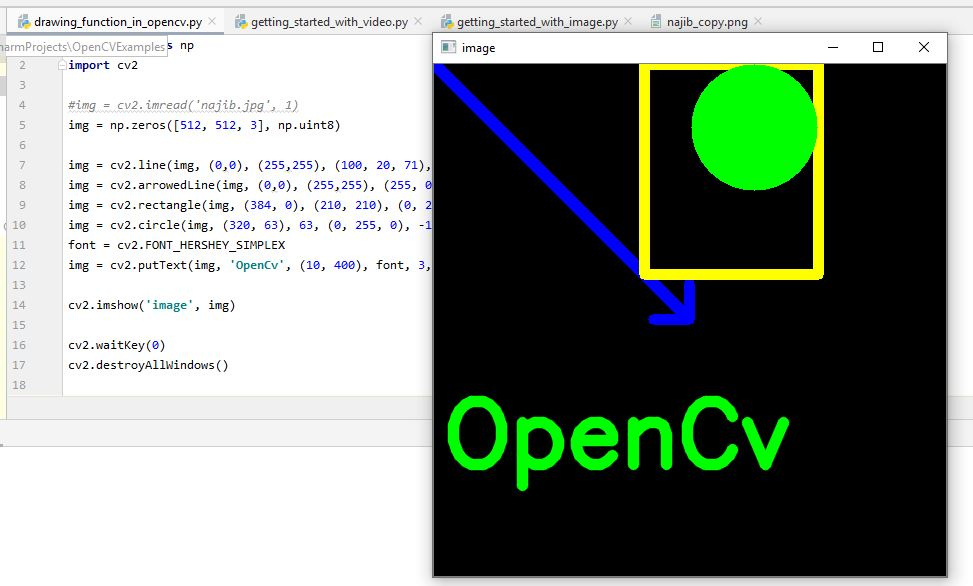
\includegraphics[scale=0.5]{figures/2,15.jpg}
\caption{Membuat Frame Numpy}
\label{contoh}
\end{figure}

Frame ini dibuat menggunakan matriks yang ada pada library numpay, kita tidak perlu lagi menghitung berapa matriksnya kita cukup gunakan zeros dan ukuran yang di butuhkan.

\newpage
\section{Ukuran Frame Menggunakan CAP PROP FRAME}
\subsection{Berubah Ukuran Frame}
\lstinputlisting{src/cv16.py}
\begin{enumerate}
	\item import cv2
	\item membuat variable cap untuk menghubungkan kamera leptop
	\item print ukuran frame lebar dan tinggi menggunakan CAP PROP FRAME WIDTH dan CAP PROP FRAME HEIGHT
	\item membuat ukuran frame baru, jika ukurannya tidak sesuai maka akan otomatis mengikuti ukutan sebelumnya.
	\item print untuk menampilkan ukuran frame saat ini
	\item membuat while yaitu perulangan membuka frame
	\item kemudian didalam perulangan tersebut terdapat frame yang membaca atau merekam video.
	\item jika kamera true merekam maka akan melakukan perintah. 
	\item buat variable dengan nama gray karna kita mau berubah kontras warnanya menjadi hitam putih, kemudian panggil cvtColor didalam frame dengan warna abu abu.
	\item kemudian buat frame dengan nama frame
	\item kemudian gunakan waitKey untuk membuat frame agar tidak langsung mati atau tertutup otomatis.
	\item release untuk menutup videocapture
	\item destroyAllWindows digunakan untuk menutup frame.
\end{enumerate}

\begin{figure}[ht]
\centering
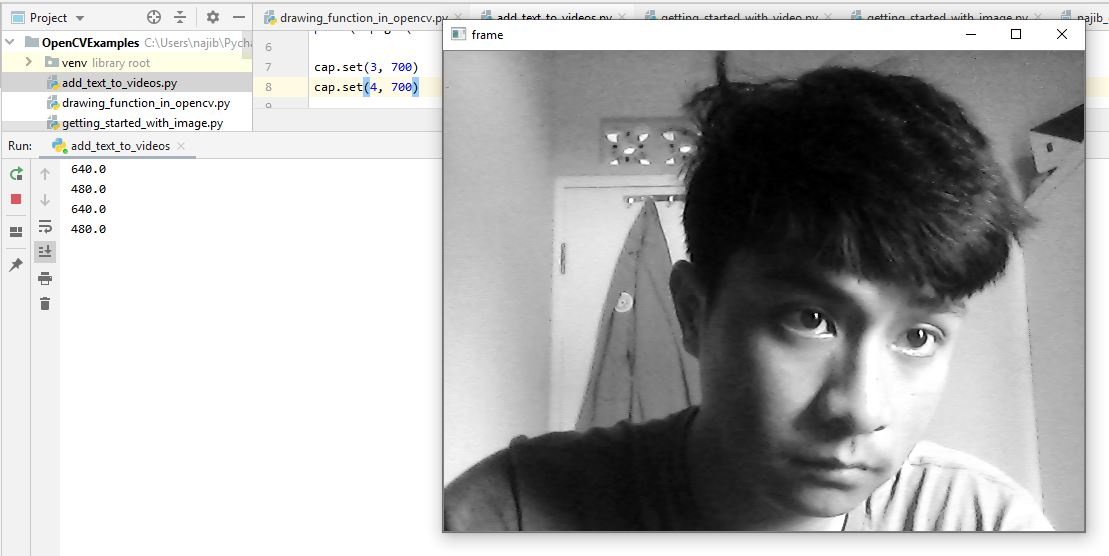
\includegraphics[scale=0.42]{figures/2,16.jpg}
\caption{Merubah ukuran frame}
\label{contoh}
\end{figure}

Pada gambar menunjukan yang di print tersebut tidak sesuai dengan yang di inginkan, karna jika kita merubah tidak sesuai dengan frame yang tertera maka akan mengikuti frame yang sebelumnya di gunakan, jadi jika ingin merubah harus sesuai.



\newpage
\section{Video Text}
\subsection{Menampilkan Text pada Frame video}
\lstinputlisting{src/cv17.py}
\begin{enumerate}
	\item import cv2
	\item membuat variable cap untuk menghubungkan kamera leptop
	\item print ukuran frame lebar dan tinggi menggunakan CAP PROP FRAME WIDTH dan CAP PROP FRAME HEIGHT
	\item membuat ukuran frame baru, jika ukurannya tidak sesuai maka akan otomatis mengikuti ukutan sebelumnya.
	\item print untuk menampilkan ukuran frame saat ini
	\item membuat while yaitu perulangan membuka frame
	\item kemudian didalam perulangan tersebut terdapat frame yang membaca atau merekam video.
	\item jika kamera true merekam maka akan melakukan perintah. 
	\item membuat font untuk tulisan pada gambar
	\item menampilkan tulisan ukuran frame
	\item menampilkan tulisan pada frame
	\item kemudian buat frame dengan nama frame
	\item kemudian gunakan waitKey untuk membuat frame agar tidak langsung mati atau tertutup otomatis.
	\item release untuk menutup videocapture
	\item destroyAllWindows digunakan untuk menutup frame.
\end{enumerate}

\begin{figure}[ht]
\centering
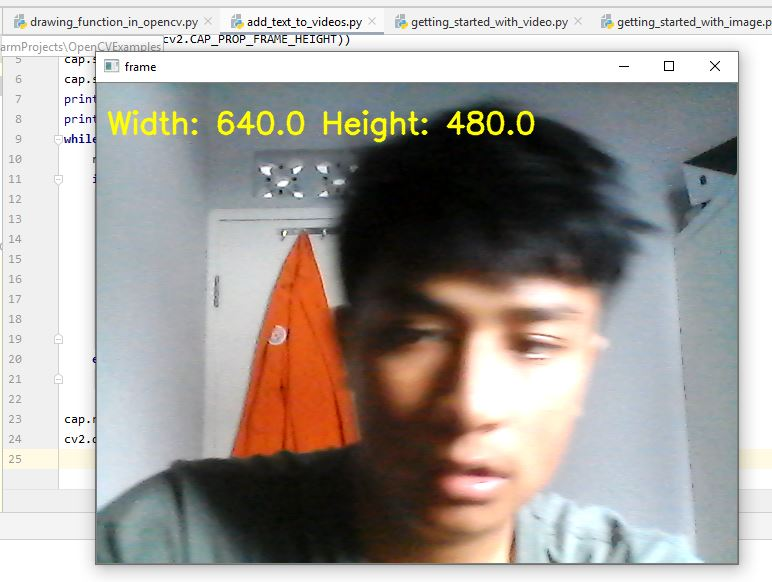
\includegraphics[scale=0.6]{figures/2,17.jpg}
\caption{Menampilkan Text pada Frame video}
\label{contoh}
\end{figure}
Pada gambar di tampilkan text dengan width ukuran lebarnya yang di panggil menggunakan print yang sebelumnya dan height tingginya, jadi code ini berguna untuk menampilkan ukuran frame yang sedang di gunakan.



\newpage
\subsection{Menampilakn waktu pada frame}
\lstinputlisting{src/cv18.py}
\begin{enumerate}
	\item import cv2
	\item import date time
	\item membuat variable cap untuk menghubungkan kamera leptop
	\item print ukuran frame lebar dan tinggi menggunakan CAP PROP FRAME WIDTH dan CAP PROP FRAME HEIGHT
	\item membuat while yaitu perulangan membuka frame
	\item kemudian didalam perulangan tersebut terdapat frame yang membaca atau merekam video.
	\item jika kamera true merekam maka akan melakukan perintah. 
	\item membuat font untuk tulisan pada gambar
	\item menampilkan tulisan ukuran frame
	\item menampilkan tulisan tanggal dan waktu pada frame
	\item kemudian buat frame dengan nama frame
	\item kemudian gunakan waitKey untuk membuat frame agar tidak langsung mati atau tertutup otomatis.
	\item release untuk menutup videocapture
	\item destroyAllWindows digunakan untuk menutup frame.
\end{enumerate}

\begin{figure}[ht]
\centering
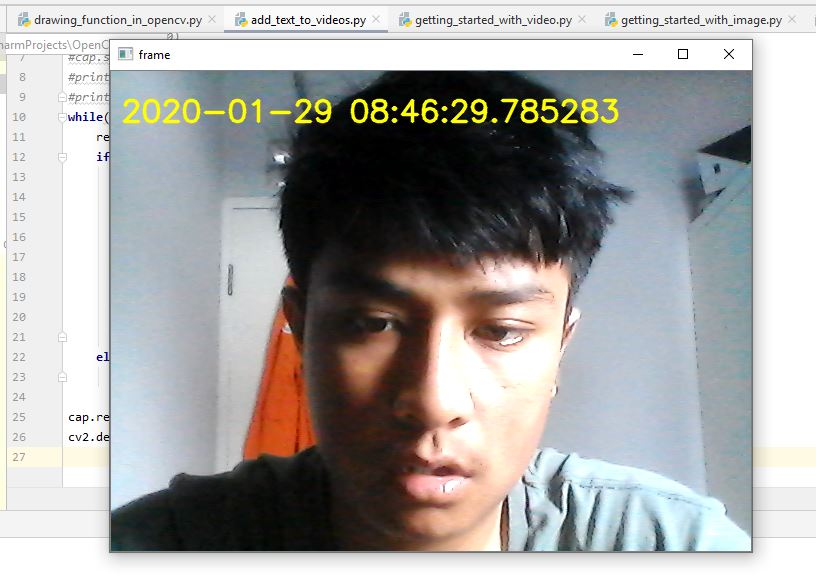
\includegraphics[scale=0.6]{figures/2,18.jpg}
\caption{Menampilakn waktu pada frame}
\label{contoh}
\end{figure}
Pada gambar di tampilkan text berwarna kuning yang menampilkan tanggal, bulan, tahun, jam hingga detik yang di ambil menggunakan library date.



\newpage
\section{Event Mouse Klik}
\subsection{Menampilkan Event}
\lstinputlisting{src/cv19.py}
\begin{enumerate}
	\item Import numpy
	\item import cv2
	\item menampilkan even event yang dapat digunakan untuk mouse klik
	\item menampilkannya dengan print
\end{enumerate}

\begin{figure}[ht]
\centering
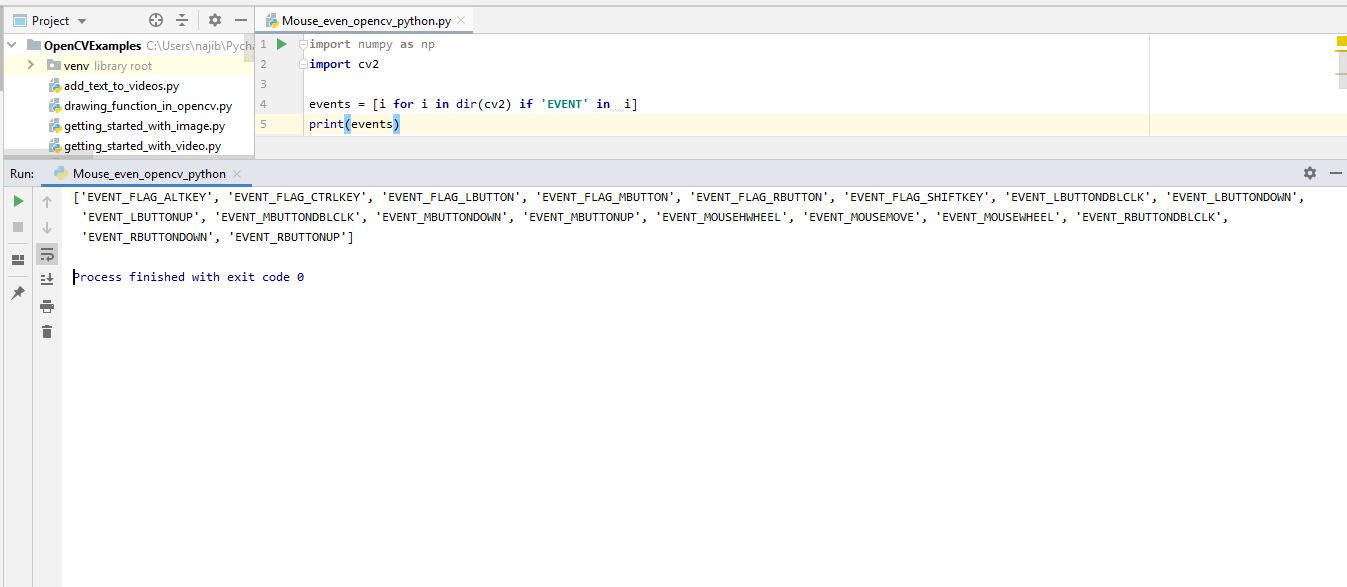
\includegraphics[scale=0.35]{figures/2,19.jpg}
\caption{Menampilkan Event}
\label{contoh}
\end{figure}



\newpage
\subsection{Event Mouse klik kiri}
\lstinputlisting{src/cv20.py}
\begin{enumerate}
	\item Import numpy
	\item import cv2
	\item buat def dengan nama click event
	\item jika mouse mengklik kiri maka akan melakukan sesuatu
	\item pada frame akan menampilkan posisi pada frame yang di klik
	\item membuat frame dengan ukuran 512 512 dengan warna hitam
	\item menampilkan frame dengan nama image
	\item memanggil fungsi klik pada mouse
	\item kemudian gunakan waitKey untuk membuat frame agar tidak langsung mati atau tertutup otomatis.
	\item destroyAllWindows digunakan untuk menutup frame.
\end{enumerate}

\newpage
\begin{figure}[ht]
\centering
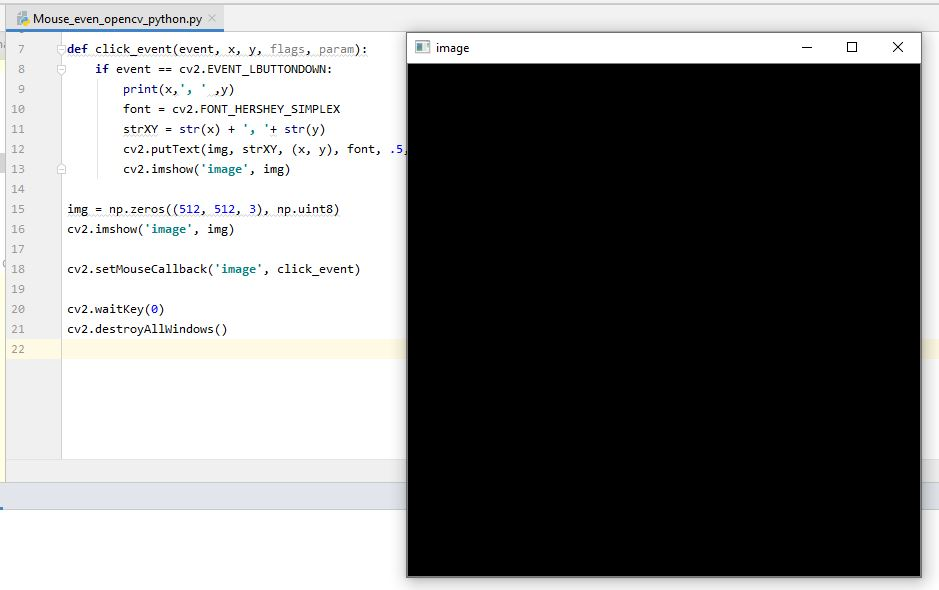
\includegraphics[scale=0.5]{figures/2,20.jpg}
\caption{Event Mouse klik kiri}
\label{contoh}
\end{figure}
Tampilan sebelum mouse kiri mengklik pada frame di bagian mana pun, gambar frame hitam karan frame tidak mengambil gambar dari mana pun

\newpage
\begin{figure}[ht]
\centering
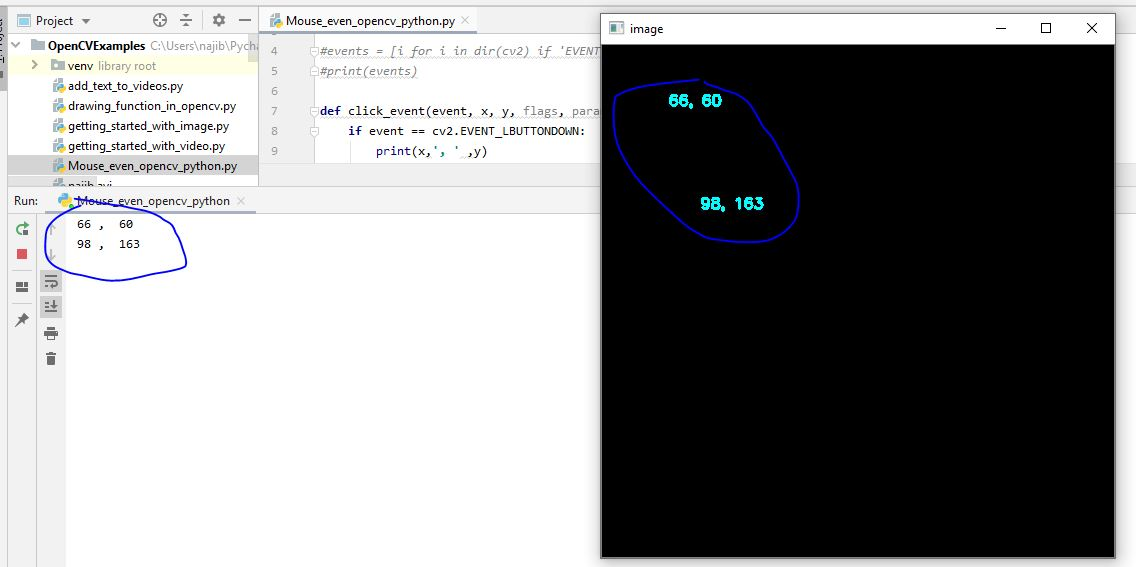
\includegraphics[scale=0.42]{figures/2,20,1.jpg}
\caption{Event Mouse klik kiri}
\label{contoh}
\end{figure}
Ketika frame di klik kiri pada bagian frame maka akan menampilkan seperti pada gambar, frame akan menampilkan lokasi x dan y dimana mouse mengklik, dan akan di print pada serial monitoe.

\newpage
\begin{figure}[ht]
\centering
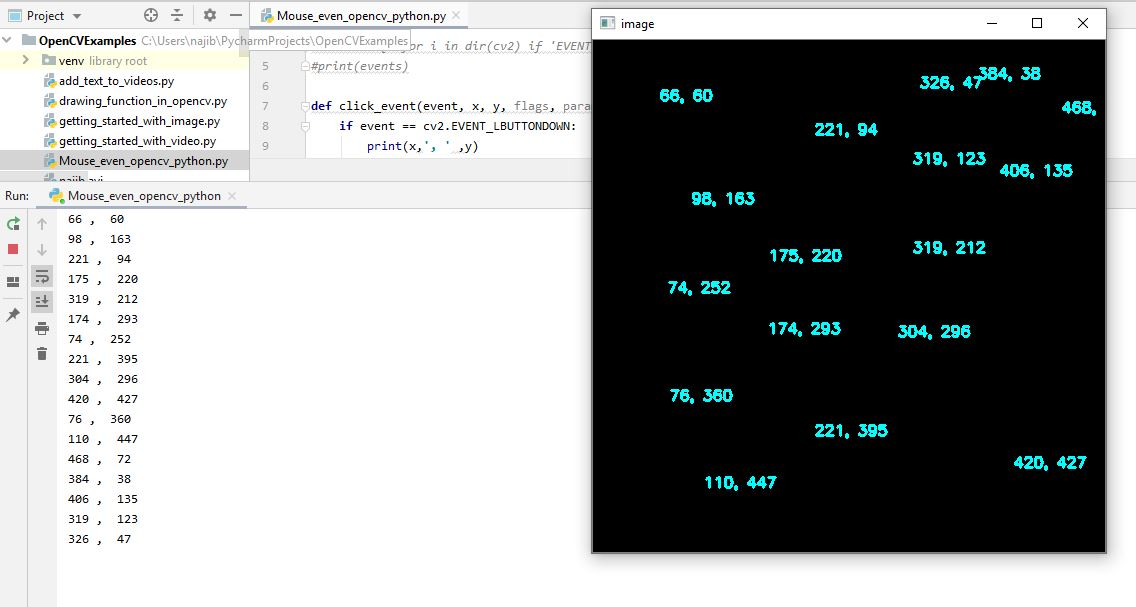
\includegraphics[scale=0.42]{figures/2,20,2.jpg}
\caption{Event Mouse klik kiri}
\label{contoh}
\end{figure}
Jika terus di klik maka frame akan terus menampilkan lokasi x dan y yang di minta oleh mouse, jika kita mengklik pada lokasi yang telah di klik pun frame akan tetap terus menampilkan sesuai permintaan mouse.



\newpage
\subsection{Event Mouse klik kiri dan kanan}
\lstinputlisting{src/cv21.py}
\begin{enumerate}
	\item Import numpy
	\item import cv2
	\item buat def dengan nama click event
	\item jika mouse mengklik kiri maka akan melakukan sesuatu
	\item pada frame akan menampilkan posisi pada frame yang di klik
	\item dan jika mouse mengklik kanan
	\item maka frame akan menampilkan nomor warna yanga ada pada frame yang di klik tersebut, terdapat 3 nomor karna menggunakan konsep bgr yaitu blue green dan red.
	\item membuat frame dengan ukuran 512 512 dengan warna hitam
	\item menampilkan frame dengan nama image
	\item memanggil fungsi klik pada mouse
	\item kemudian gunakan waitKey untuk membuat frame agar tidak langsung mati atau tertutup otomatis.
	\item destroyAllWindows digunakan untuk menutup frame.
\end{enumerate}

\begin{figure}[ht]
\centering
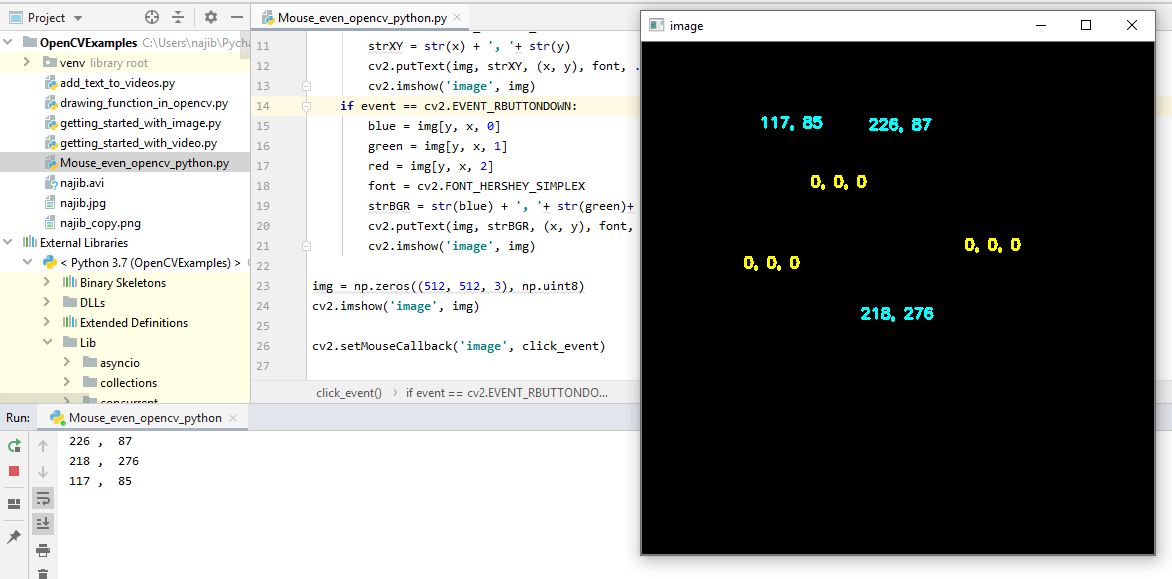
\includegraphics[scale=0.4]{figures/2,21.jpg}
\caption{Event Mouse klik kiri dan kanan}
\label{contoh}
\end{figure}
Pada gambar menampilkan koordinat x dan y untuk yang berwarna biru yang sudah di jelaskan pada section sebelumnya, sedangkan yang berwarna kuning berguna untuk menampilkan nomor warna pada frame karan pada frame berwarna hitam dan nomor wara untuk hitam adalah 0,0,0 maka frame menampilkan seperti pada gambar.



\newpage
\subsection{Event Mouse klik kiri dan kanan pada gambar yang dipangggil}
\lstinputlisting{src/cv22.py}
\begin{enumerate}
	\item Import numpy
	\item import cv2
	\item buat def dengan nama click event
	\item jika mouse mengklik kiri maka akan melakukan sesuatu
	\item pada frame akan menampilkan posisi pada frame yang di klik
	\item dan jika mouse mengklik kanan
	\item maka frame akan menampilkan nomor warna yanga ada pada frame yang di klik tersebut, terdapat 3 nomor karna menggunakan konsep bgr yaitu blue green dan red.
	\item memanggil gambar untuk di taruh pada frame yang telah di buat
	\item menampilkan frame dengan nama image
	\item memanggil fungsi klik pada mouse
	\item kemudian gunakan waitKey untuk membuat frame agar tidak langsung mati atau tertutup otomatis.
	\item destroyAllWindows digunakan untuk menutup frame.
\end{enumerate}

\newpage
\begin{figure}[ht]
\centering
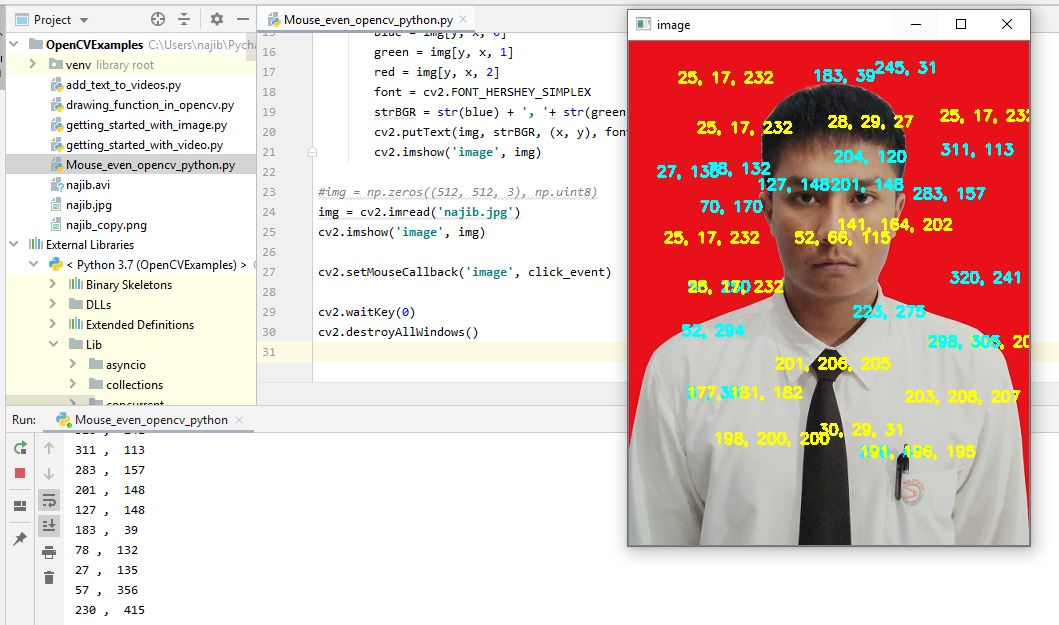
\includegraphics[scale=0.47]{figures/2,22.jpg}
\caption{Event Mouse klik kiri dan kanan pada gambar yang dipangggil}
\label{contoh}
\end{figure}
Pada gambar menampilkan koordinat x dan y untuk yang berwarna biru yang sudah di jelaskan pada section sebelumnya, sedangkan yang berwarna kuning berguna untuk menampilkan nomor warna pada frame, frame akan menampilkan nomor warna sesuai warna yang ada pada mouse yang di klik.




\newpage
\subsection{Event Mouse klik kiri membuat titik dan garis}
\lstinputlisting{src/cv23.py}
\begin{enumerate}
	\item Import numpy
	\item import cv2
	\item buat def dengan nama click event
	\item jika mouse mengklik kiri maka akan melakukan sesuatu
	\item pada frame akan membuat sebuah titik berwarna merah sesuai lokasi mengklik frame
	\item jika titik tersebut lebih dari sama dengan 2 maka setiap titik yang terakhir akan terhubung satu sama lain.
	\item menampilkan frame dengan nama image
	\item gambar pada frame berwarna hitam
	\item menampilkan frame kembali
	\item point menghilang setelah berubah menjadi garis atau line
	\item memanggil fungsi klik pada mouse
	\item kemudian gunakan waitKey untuk membuat frame agar tidak langsung mati atau tertutup otomatis.
	\item destroyAllWindows digunakan untuk menutup frame.
\end{enumerate}

\newpage
\begin{figure}[ht]
\centering
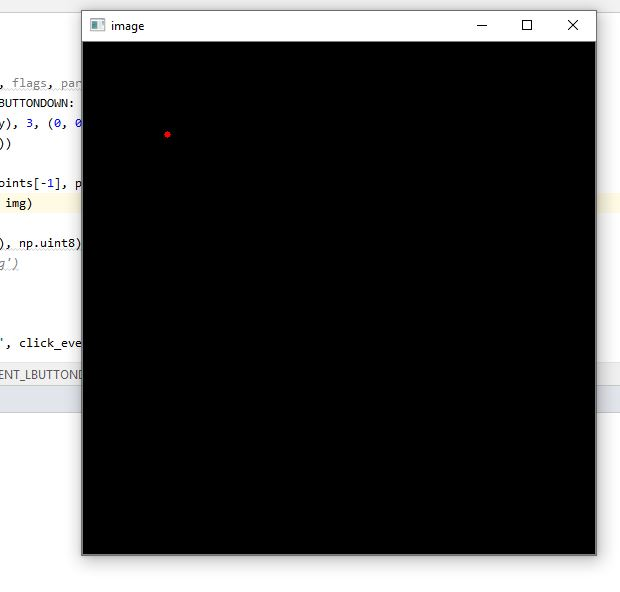
\includegraphics[scale=0.7]{figures/2,23.jpg}
\caption{Event Mouse klik kiri membuat titik dan garis}
\label{contoh}
\end{figure}
Ketika frame mengklik pada kiri pada frame maka frame akan menampilkan titik berwarna merah sesuai lokasi mouse mengklik frame.

\newpage
\begin{figure}[ht]
\centering
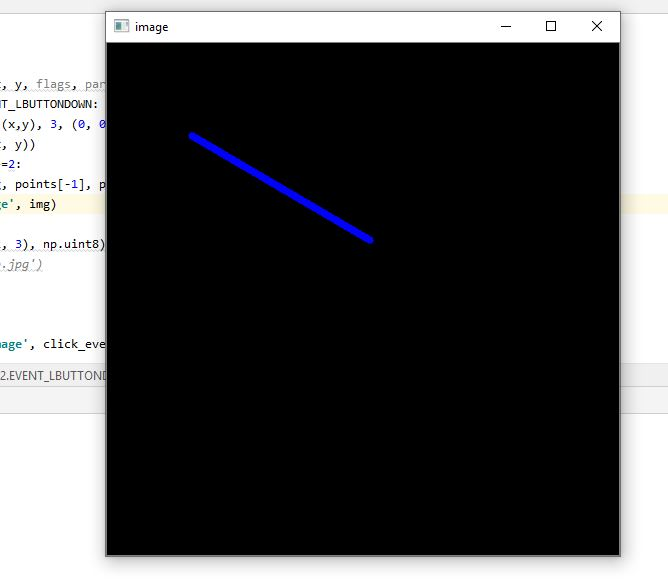
\includegraphics[scale=0.7]{figures/2,23,1.jpg}
\caption{Event Mouse klik kiri membuat titik dan garis}
\label{contoh}
\end{figure}
Ketika mouse mengklik kembali pada frame di lokasi yang berbeda maka titik merah yang pertama akan menghilang dan pada titik yang pertama akan menghubungkan ke titik yang ke dua menjadi sebuah garis.

\newpage
\begin{figure}[ht]
\centering
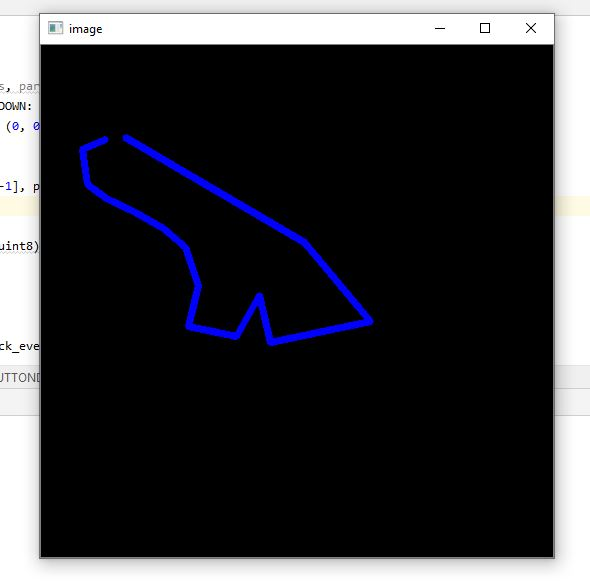
\includegraphics[scale=0.7]{figures/2,23,2.jpg}
\caption{Event Mouse klik kiri membuat titik dan garis}
\label{contoh}
\end{figure}
Jadi jika titik merah lebih dari sama dengan 2 maka titik merah akan menghilang dan akan menghubungkan dari titik satu ke titik yang kedua jika mouse mengklik kembali menjadi titik yang ke tiga maka titi yang terakhir akan menghubungkan ke titik yang baru.



\newpage
\subsection{Membuat frame warna sesuai klik}
\lstinputlisting{src/cv24.py}
\begin{enumerate}
	\item Import numpy
	\item import cv2
	\item buat def dengan nama click event
	\item jika mouse mengklik kiri maka akan melakukan sesuatu
	\item warna biru di deklarasikan dengan 0
	\item warna hijau di deklarasikan dengan 1
	\item warna merah di deklarasikan dengan 2
	\item membuat lingkaran kecil berwarna merah
	\item membuat warna sesuai lokasi frame yang di klik harus sesuai dengan warna yang di klik
	\item memanggil gambar
	\item menampilkan frame kembali
	\item point menghilang setelah berubah menjadi garis atau line
	\item memanggil fungsi klik pada mouse
	\item kemudian gunakan waitKey untuk membuat frame agar tidak langsung mati atau tertutup otomatis.
	\item destroyAllWindows digunakan untuk menutup frame.

\end{enumerate}

\begin{figure}[ht]
\centering
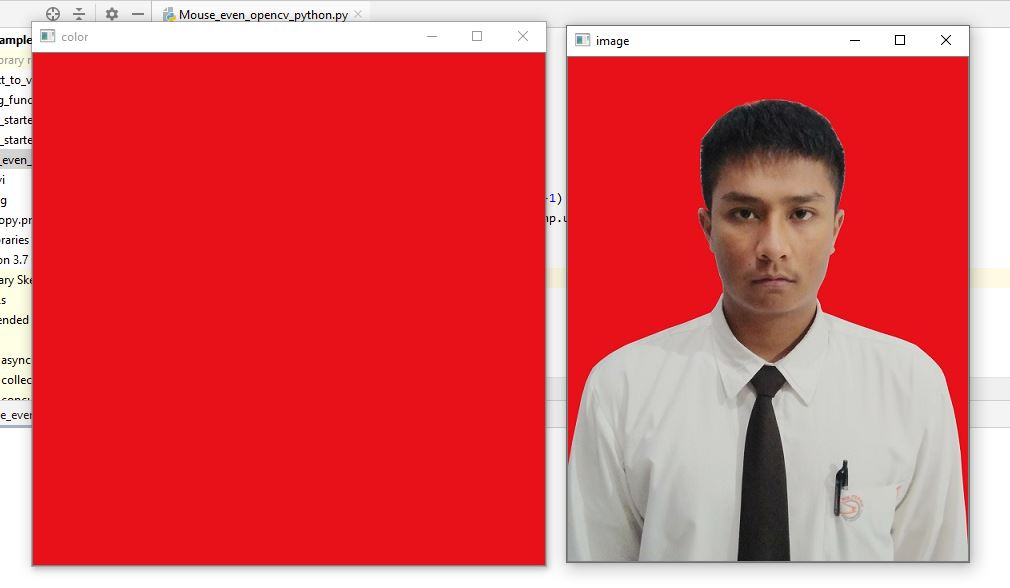
\includegraphics[scale=0.45]{figures/2,24.jpg}
\caption{Membuat frame warna sesuai klik}
\label{contoh}
\end{figure}

\newpage
\begin{figure}[ht]
\centering
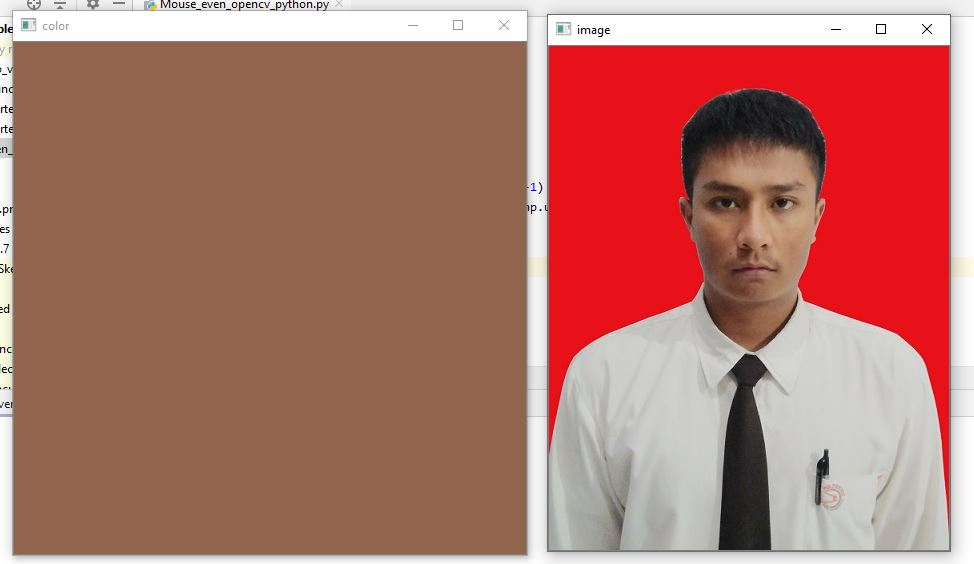
\includegraphics[scale=0.4]{figures/2,24,1.jpg}
\caption{Membuat frame warna sesuai klik}
\label{contoh}
\end{figure}

\begin{figure}[ht]
\centering
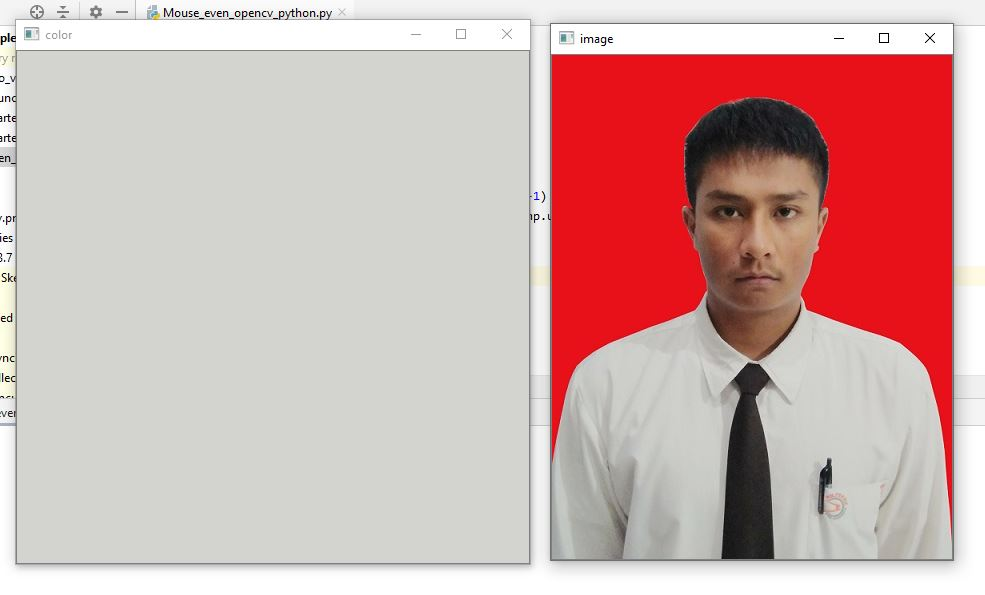
\includegraphics[scale=0.4]{figures/2,24,2.jpg}
\caption{Membuat frame warna sesuai klik}
\label{contoh}
\end{figure}



\newpage
\subsection{Membuat frame warna sesuai klik 2}
\lstinputlisting{src/cv25.py}
\begin{enumerate}
	\item Import numpy
	\item import cv2
	\item buat def dengan nama click event
	\item jika mouse mengklik kiri maka akan melakukan sesuatu
	\item warna biru di deklarasikan dengan 0
	\item warna hijau di deklarasikan dengan 1
	\item warna merah di deklarasikan dengan 2
	\item membuat lingkaran kecil berwarna merah
	\item membuat warna sesuai lokasi frame yang di klik harus sesuai dengan warna yang di klik
	\item menggunakan gambar hitam
	\item menampilkan frame kembali
	\item point menghilang setelah berubah menjadi garis atau line
	\item memanggil fungsi klik pada mouse
	\item kemudian gunakan waitKey untuk membuat frame agar tidak langsung mati atau tertutup otomatis.
	\item destroyAllWindows digunakan untuk menutup frame.
\end{enumerate}

\begin{figure}[ht]
\centering
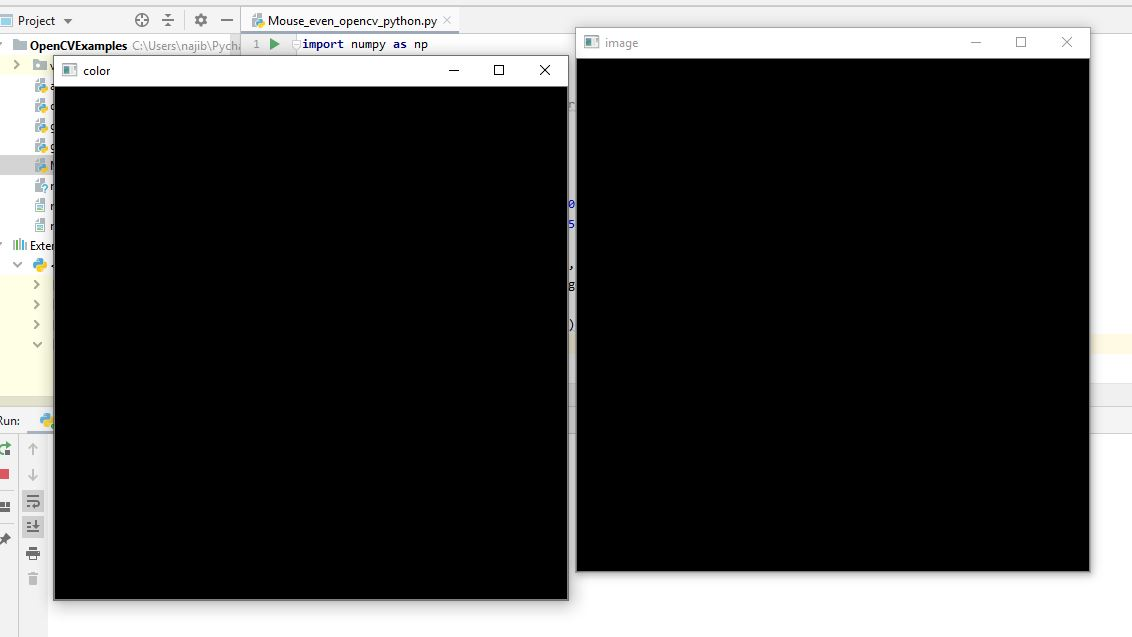
\includegraphics[scale=0.4]{figures/2,25.jpg}
\caption{Membuat frame warna sesuai klik 2}
\label{contoh}
\end{figure}



\newpage
\subsection{Menampilkan Shape, size, dan dtype}
\lstinputlisting{src/cv26.py}
\begin{enumerate}
	\item import numpy
	\item import cv2
	\item mengambil gambar dari file 
	\item menampilkan ukuran lebar dan tingi frame
	\item menampilkan ukuran dari frame
	\item menampilkan jenis gambar yang ada pada frame
	\item membagi tiap warna pada gambar
	\item menampilkan frame dengan nama image 
	\item kemudian gunakan waitKey untuk membuat frame agar tidak langsung mati atau tertutup otomatis.
	\item destroyAllWindows digunakan untuk menutup frame.
\end{enumerate}

\newpage
\begin{figure}[ht]
\centering
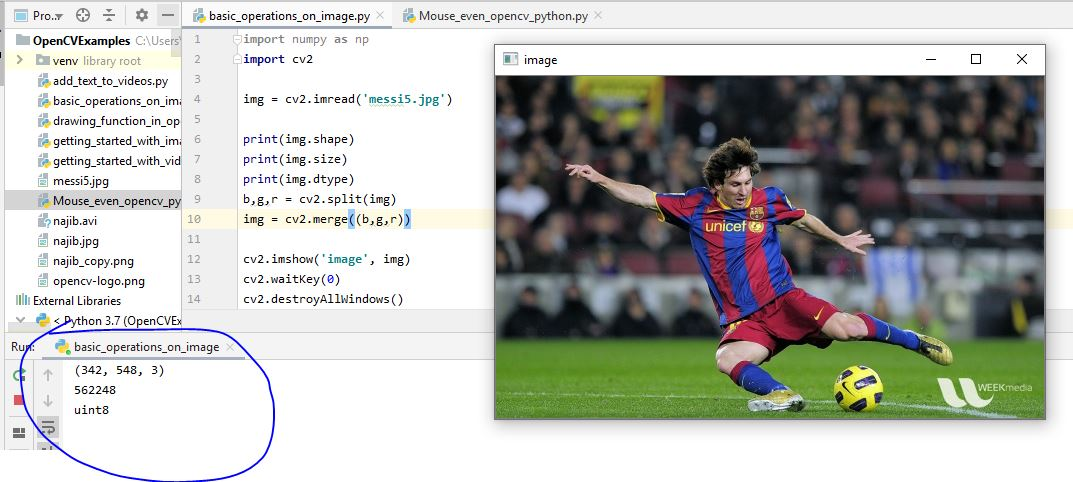
\includegraphics[scale=0.45]{figures/2,26.jpg}
\caption{Menampilkan Shape, size, dan dtype}
\label{contoh}
\end{figure}



\newpage
\subsection{Mengcopy gambar di dalam satu frame}
\lstinputlisting{src/cv27.py}
\begin{enumerate}
	\item import numpy
	\item import cv2
	\item mengambil gambar dari file 
	\item menampilkan ukuran lebar dan tingi frame
	\item menampilkan ukuran dari frame
	\item menampilkan jenis gambar yang ada pada frame
	\item membagi tiap warna pada gambar
	\item membuat variabel baru untuk mengcopy gambar yang teretak pada titik titik yang di tentukan
	\item menempatkan gambar yang telah di copy ke titik baru yang di tentukan
	\item menampilkan frame dengan nama image 
	\item kemudian gunakan waitKey untuk membuat frame agar tidak langsung mati atau tertutup otomatis.
	\item destroyAllWindows digunakan untuk menutup frame.
\end{enumerate}

\newpage
\begin{figure}[ht]
\centering
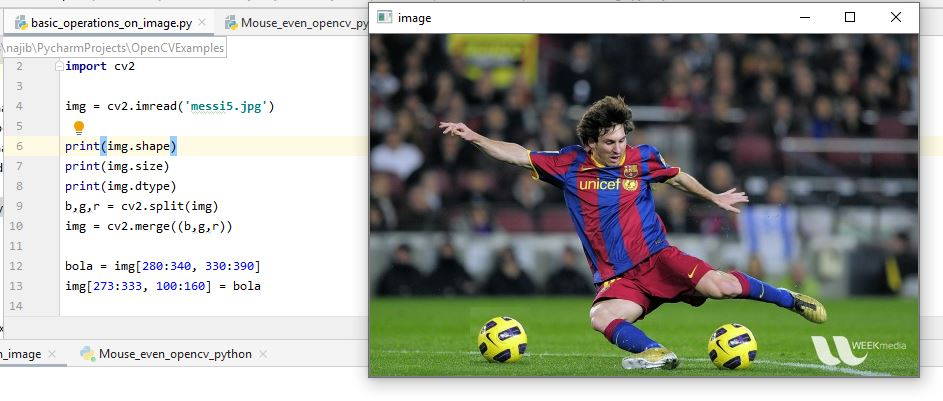
\includegraphics[scale=0.5]{figures/2,27.jpg}
\caption{Mengcopy gambar di dalam satu frame}
\label{contoh}
\end{figure}



\newpage
\section{Menyatukan gambar dalam satu frame}
\subsection{Menyatukan 2 gambar dalam 1 frame}
\lstinputlisting{src/cv28.py}
\begin{enumerate}
	\item import numpy
	\item import cv2
	\item mengambil gambar dari file 
	\item mengambil gambar kedua untuk di satukan dalam satu frame
	\item menampilkan ukuran lebar dan tingi frame
	\item menampilkan ukuran dari frame
	\item menampilkan jenis gambar yang ada pada frame
	\item membagi tiap warna pada gambar
	\item mengubah ukuran gambar yang ke1 harus sama satu sama lain
	\item mengubah ukuran gambar yang ke2 harus sama satu sama lain
	\item menggabungkan gambar menggunakan add dan sebutkan kedua gambar
	\item menampilkan frame dengan nama image dan panggil variable dst
	\item kemudian gunakan waitKey untuk membuat frame agar tidak langsung mati atau tertutup otomatis.
	\item destroyAllWindows digunakan untuk menutup frame.
\end{enumerate}

\newpage
\begin{figure}[ht]
\centering
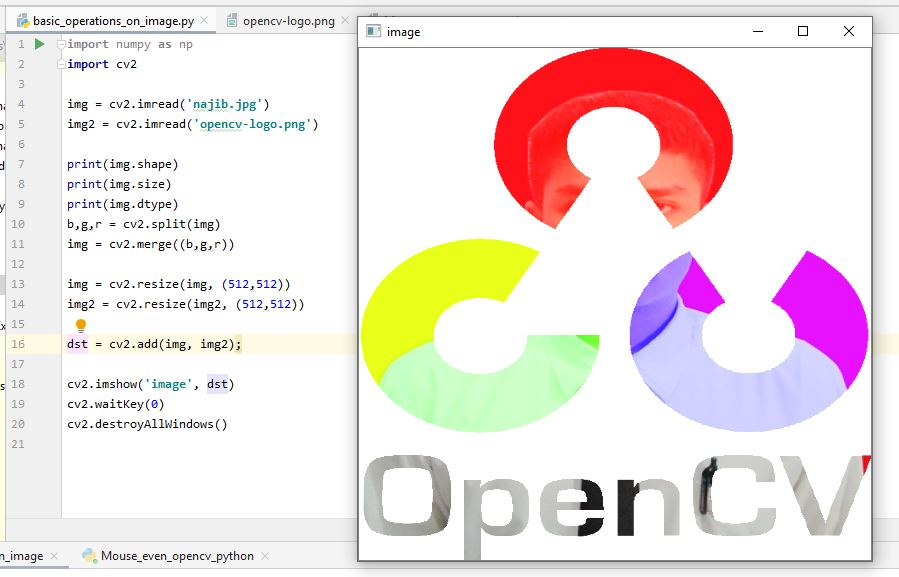
\includegraphics[scale=0.5]{figures/2,28.jpg}
\caption{Menyatukan 2 gambar dalam 1 frame}
\label{contoh}
\end{figure}



\newpage
\subsection{Menggabungkan 2 gambar dengan kontras transparan}
\lstinputlisting{src/cv29.py}
\begin{enumerate}
	\item import numpy
	\item import cv2
	\item mengambil gambar dari file 
	\item mengambil gambar kedua untuk di satukan dalam satu frame
	\item menampilkan ukuran lebar dan tingi frame
	\item menampilkan ukuran dari frame
	\item menampilkan jenis gambar yang ada pada frame
	\item membagi tiap warna pada gambar
	\item mengubah ukuran gambar yang ke1 harus sama satu sama lain
	\item mengubah ukuran gambar yang ke2 harus sama satu sama lain
	\item untuk kontras ransparan gunakan addWeighted dan tentukan kontrasnya sesuai gambar
	\item menampilkan frame dengan nama image dan panggil variable dst
	\item kemudian gunakan waitKey untuk membuat frame agar tidak langsung mati atau tertutup otomatis.
	\item destroyAllWindows digunakan untuk menutup frame.
\end{enumerate}

\newpage
\begin{figure}[ht]
\centering
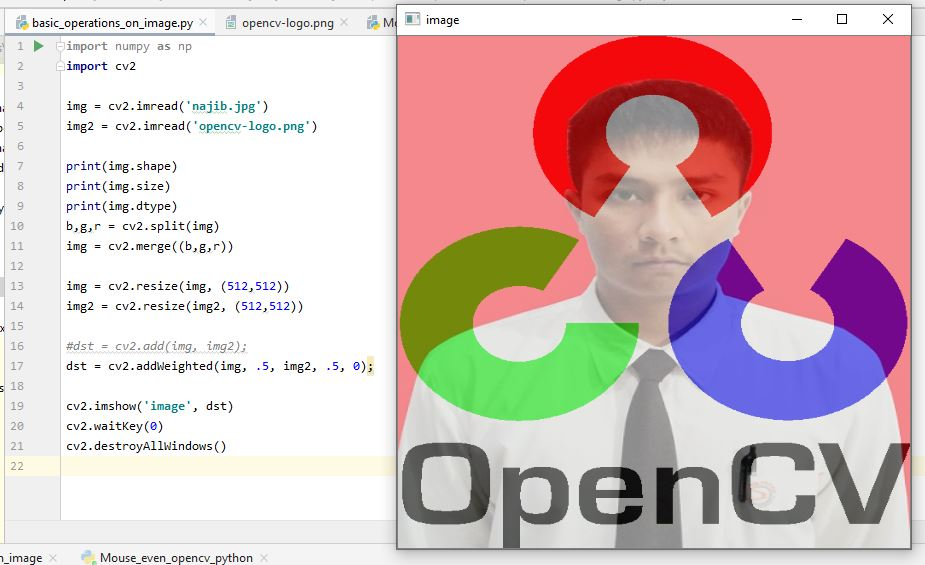
\includegraphics[scale=0.5]{figures/2,29.jpg}
\caption{Menggabungkan 2 gambar dengan kontras transparan}
\label{contoh}
\end{figure}



\newpage
\section{Trackbar}
\subsection{Membuat Trackbar}
\lstinputlisting{src/cv30.py}
\begin{enumerate}
	\item import numpy
	\item import cv
	\item membuat variable untuk menampilkan
	\item membuat gambar hitam menggunakan zeros dan ukuran frame yang di inginkan
	\item buat jendela dengan nama image
	\item membuat Trackbar B digunakan untuk kontras warna biru dari 0 sampai 255, kemudian data di tampilkan menggunakan nothing sesuai kursor yang di geser
	\item membuat Trackbar G digunakan untuk kontras warna hijau dari 0 sampai 255, kemudian data di tampilkan menggunakan nothing sesuai kursor yang di geser
	\item membuat Trackbar R digunakan untuk kontras warna merah dari 0 sampai 255, kemudian data di tampilkan menggunakan nothing sesuai kursor yang di geser
	\item membuat pengulangan 
	\item menampilkan frame dengan isi frame img yang telah di buat
	\item membuat waitKey jika sama dengan 27 maka akan berakhir
	\item destroyAllWindows digunakan untuk menutup frame.
\end{enumerate}

\begin{figure}[ht]
\centering
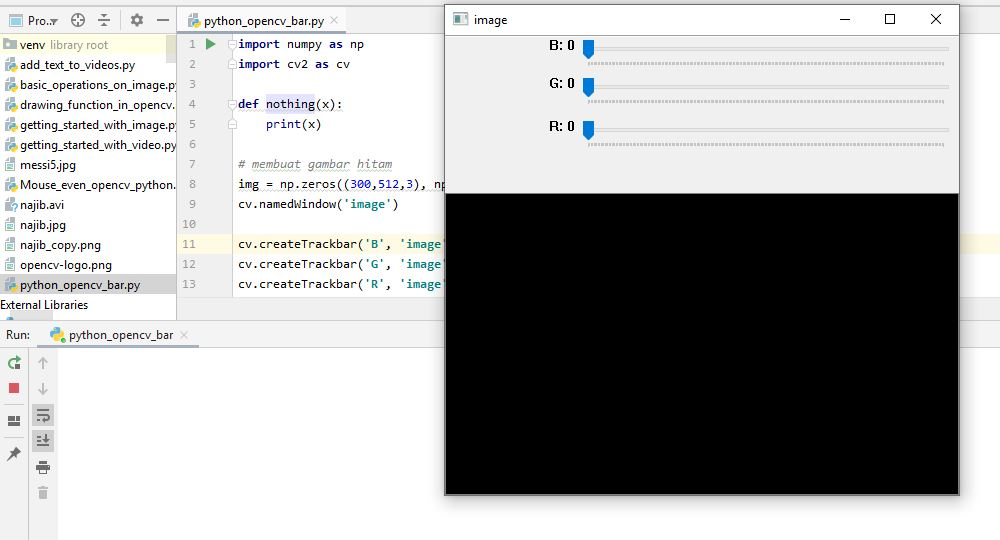
\includegraphics[scale=0.45]{figures/2,30.jpg}
\caption{Membuat Trackbar}
\label{contoh}
\end{figure}

\newpage
\begin{figure}[ht]
\centering
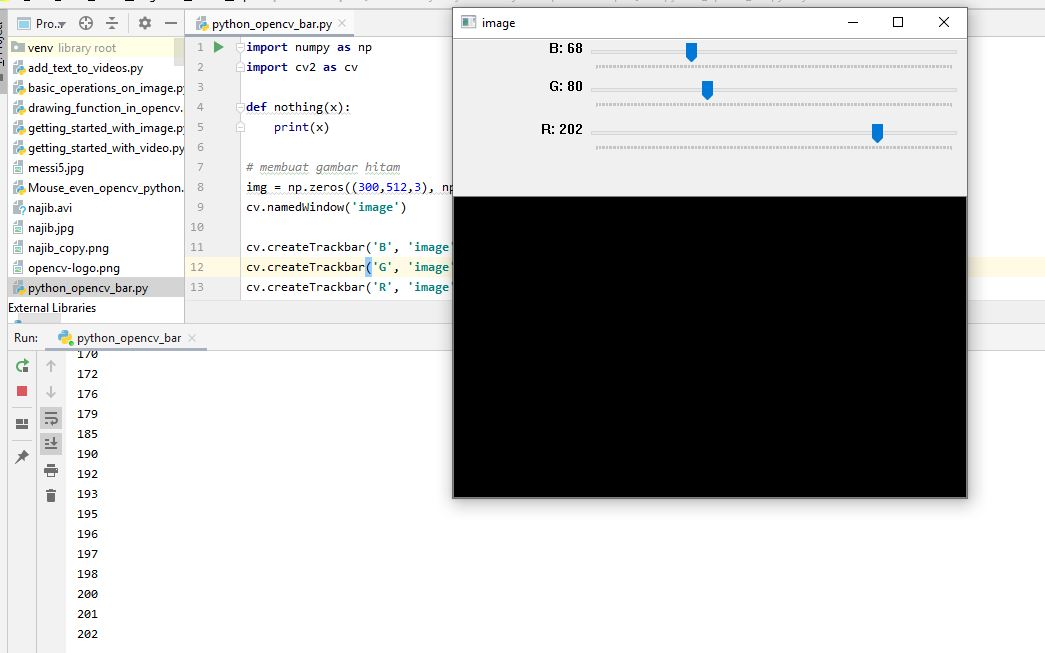
\includegraphics[scale=0.45]{figures/2,30,1.jpg}
\caption{Membuat Trackbar}
\label{contoh}
\end{figure}



\newpage
\subsection{Membuat Trackbar dengan fungsi warna}
\lstinputlisting{src/cv31.py}
\begin{enumerate}
	\item import numpy
	\item import cv
	\item membuat variable untuk menampilkan
	\item membuat gambar hitam menggunakan zeros dan ukuran frame yang di inginkan
	\item buat jendela dengan nama image
	\item membuat Trackbar B digunakan untuk kontras warna biru dari 0 sampai 255, kemudian data di tampilkan menggunakan nothing sesuai kursor yang di geser
	\item membuat Trackbar G digunakan untuk kontras warna hijau dari 0 sampai 255, kemudian data di tampilkan menggunakan nothing sesuai kursor yang di geser
	\item membuat Trackbar R digunakan untuk kontras warna merah dari 0 sampai 255, kemudian data di tampilkan menggunakan nothing sesuai kursor yang di geser
	\item membuat pengulangan 
	\item menampilkan frame dengan isi frame img yang telah di buat
	\item membuat waitKey jika sama dengan 27 maka akan berakhir
	\item untuk mengisi Trackbar sesuai warna kontras warna yang di tentukan kita gunakan getTrackbarPos dan definisikan di awal sesuai warnanya biru hijau dan merah 
	\item kemudian definisikan kalau variable bgr tersebut adalah warna biru hijau dan merah
	\item destroyAllWindows digunakan untuk menutup frame.
\end{enumerate}

\begin{figure}[ht]
\centering
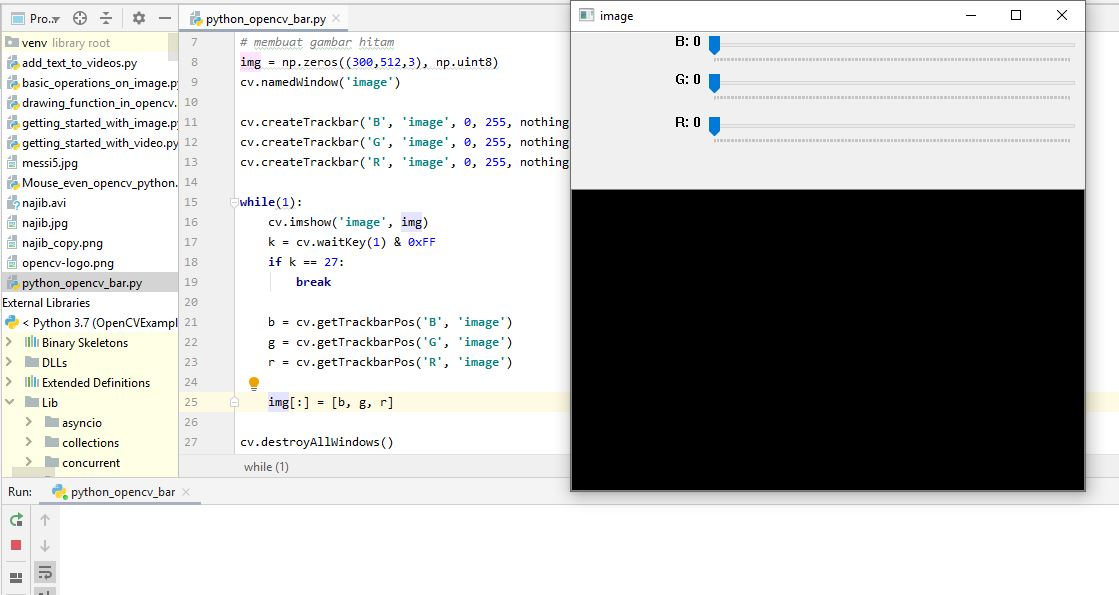
\includegraphics[scale=0.42]{figures/2,31.jpg}
\caption{Membuat Trackbar dengan fungsi warna}
\label{contoh}
\end{figure}

\newpage
\begin{figure}[ht]
\centering
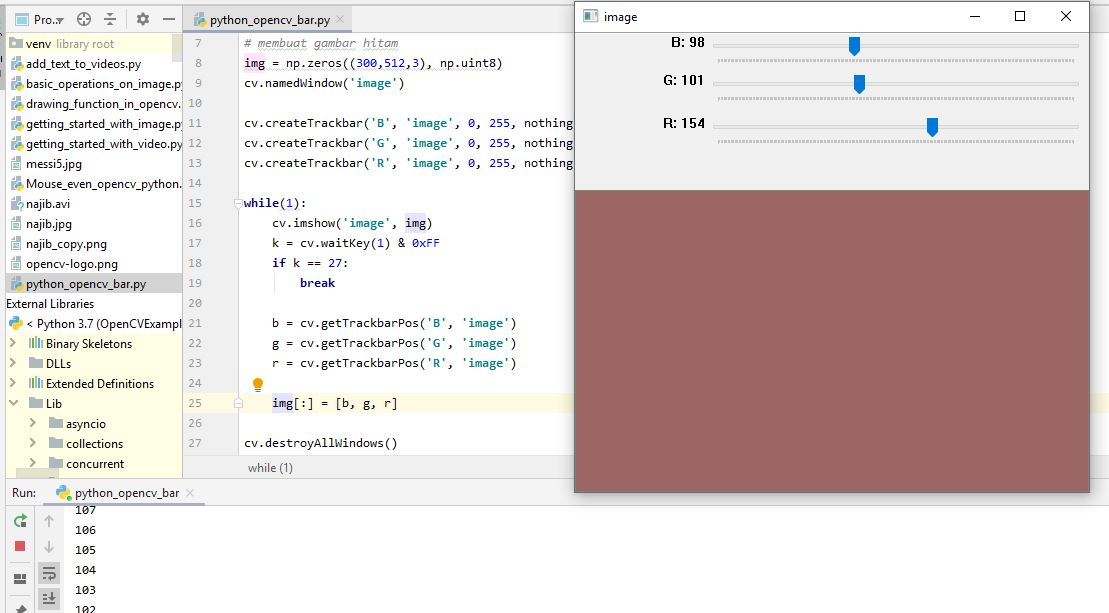
\includegraphics[scale=0.42]{figures/2,31,1.jpg}
\caption{Membuat Trackbar dengan fungsi warna}
\label{contoh}
\end{figure}



\newpage
\subsection{Membuat Trackbar ON dan OFF}
\lstinputlisting{src/cv32.py}
\begin{enumerate}
	\item import numpy
	\item import cv
	\item membuat variable untuk menampilkan
	\item membuat gambar hitam menggunakan zeros dan ukuran frame yang di inginkan
	\item buat jendela dengan nama image
	\item membuat Trackbar B digunakan untuk kontras warna biru dari 0 sampai 255, kemudian data di tampilkan menggunakan nothing sesuai kursor yang di geser
	\item membuat Trackbar G digunakan untuk kontras warna hijau dari 0 sampai 255, kemudian data di tampilkan menggunakan nothing sesuai kursor yang di geser
	\item membuat Trackbar R digunakan untuk kontras warna merah dari 0 sampai 255, kemudian data di tampilkan menggunakan nothing sesuai kursor yang di geser
	\item membuat tampilan on dan off
	\item membuat Trackbar on dan off dari 0 sampai 1, kemudian data di tampilkan menggunakan nothing sesuai kursor yang di geser
	\item membuat pengulangan 
	\item menampilkan frame dengan isi frame img yang telah di buat
	\item membuat waitKey jika sama dengan 27 maka akan berakhir
	\item untuk mengisi Trackbar sesuai warna kontras warna yang di tentukan kita gunakan getTrackbarPos dan definisikan di awal sesuai warnanya biru hijau dan merah 
	\item kemudian jika keadaan of maka tidak akan ada kontras warna jika kursor biru hijau dan merah di gerakan, dan jika kursor sudah on maka warna akan menyesuaikan
	\item destroyAllWindows digunakan untuk menutup frame.
\end{enumerate}

\newpage
\begin{figure}[ht]
\centering
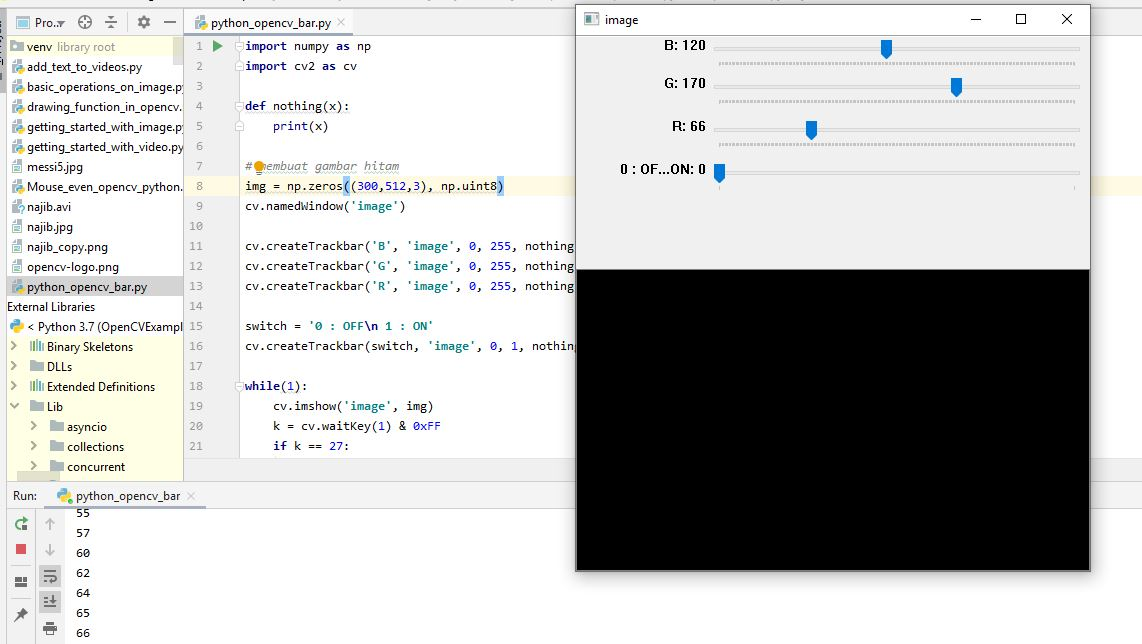
\includegraphics[scale=0.42]{figures/2,32.jpg}
\caption{Membuat Trackbar ON dan OFF}
\label{contoh}
\end{figure}

\newpage
\begin{figure}[ht]
\centering
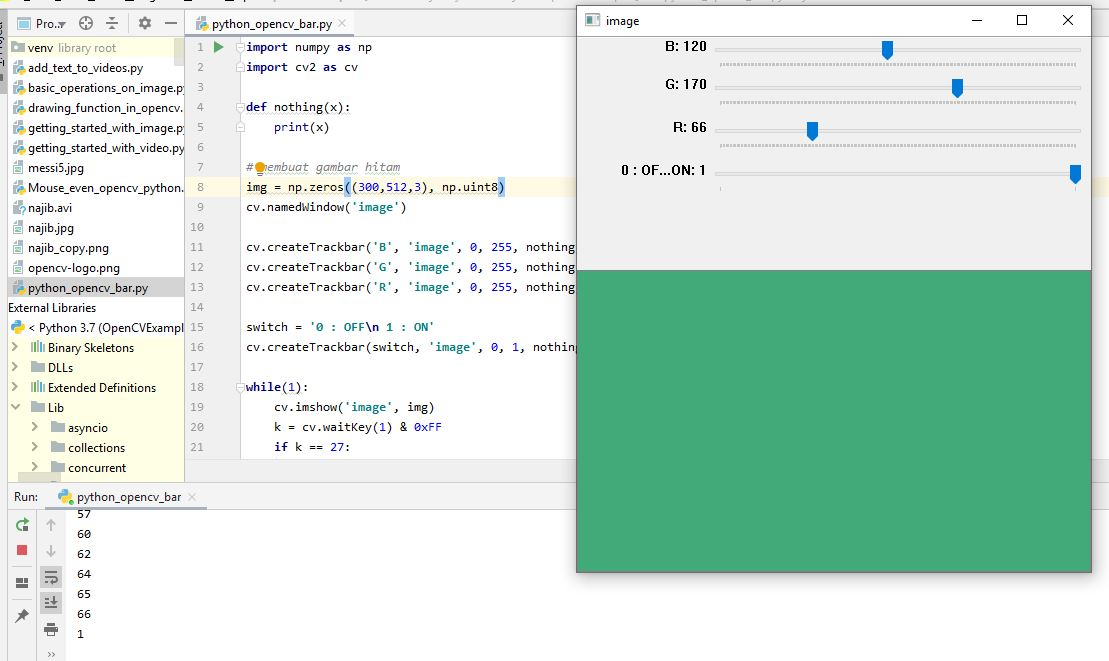
\includegraphics[scale=0.42]{figures/2,32,1.jpg}
\caption{Membuat Trackbar ON dan OFF}
\label{contoh}
\end{figure}



\newpage
\subsection{Trackbar menampilkan text kontras}
\lstinputlisting{src/cv33.py}
\begin{enumerate}
	\item import numpy
	\item import cv
	\item membuat variable untuk menampilkan
	\item buat jendela dengan nama image
	\item membuat Trackbar CP dari 10 sampai 400, kemudian data di tampilkan menggunakan nothing sesuai kursor yang di geser
	\item membuat tampilan on dan off
	\item membuat Trackbar on dan off dari 0 sampai 1, kemudian data di tampilkan menggunakan nothing sesuai kursor yang di geser
	\item membuat pengulangan 
	\item menampilkan frame dengan isi frame img yang telah dipanggil dari file
	\item mengambil fungsi Trackbar menggunakan getTrackbarPos pada CP
	\item kemudian atur font text yang akan di gunakan
	\item atur text ukuran, wrna, font, dan mengambil string dari variable pos
	\item membuat waitKey jika sama dengan 27 maka akan berakhir
	\item kemudian mengambil fungsi trackbar kedua yaitu switch 
	\item jika switch 0 maka tidak akan mengubah apapun
	\item jika switch 1 maka akan merubah kontras warna menjadi abu abu
	\item menampilkan frame
	\item destroyAllWindows digunakan untuk menutup frame.
\end{enumerate}

\newpage
\begin{figure}[ht]
\centering
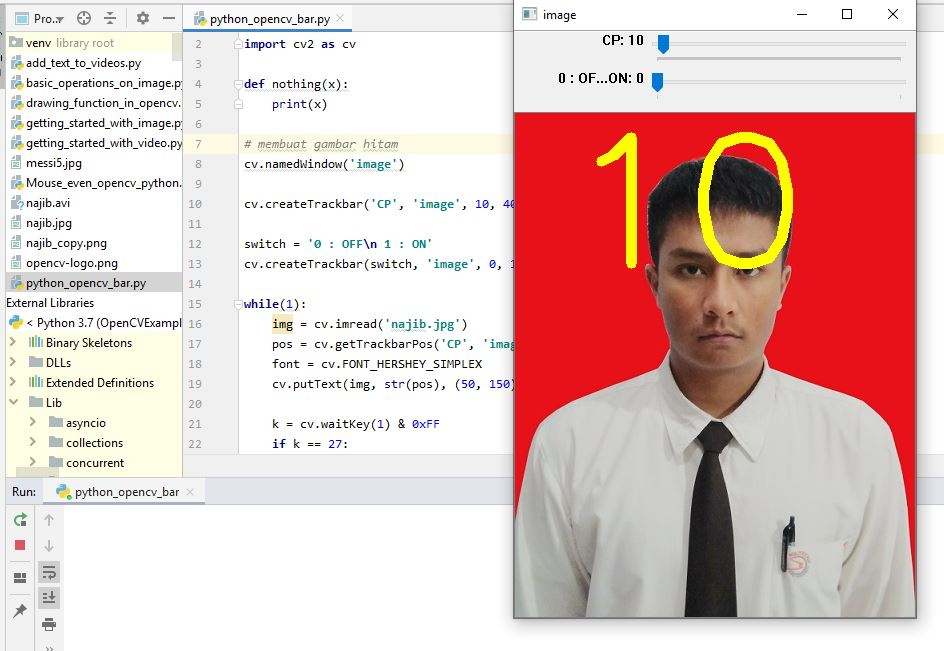
\includegraphics[scale=0.5]{figures/2,33.jpg}
\caption{Trackbar menampilkan text kontras}
\label{contoh}
\end{figure}

\newpage
\begin{figure}[ht]
\centering
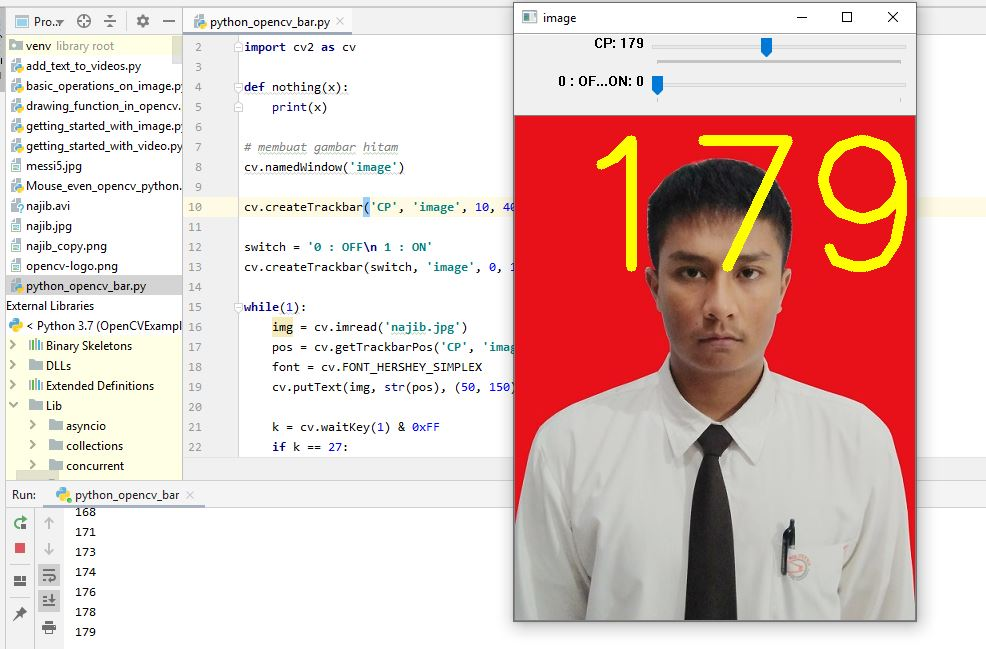
\includegraphics[scale=0.5]{figures/2,33,1.jpg}
\caption{Trackbar menampilkan text kontras}
\label{contoh}
\end{figure}

\newpage
\begin{figure}[ht]
\centering
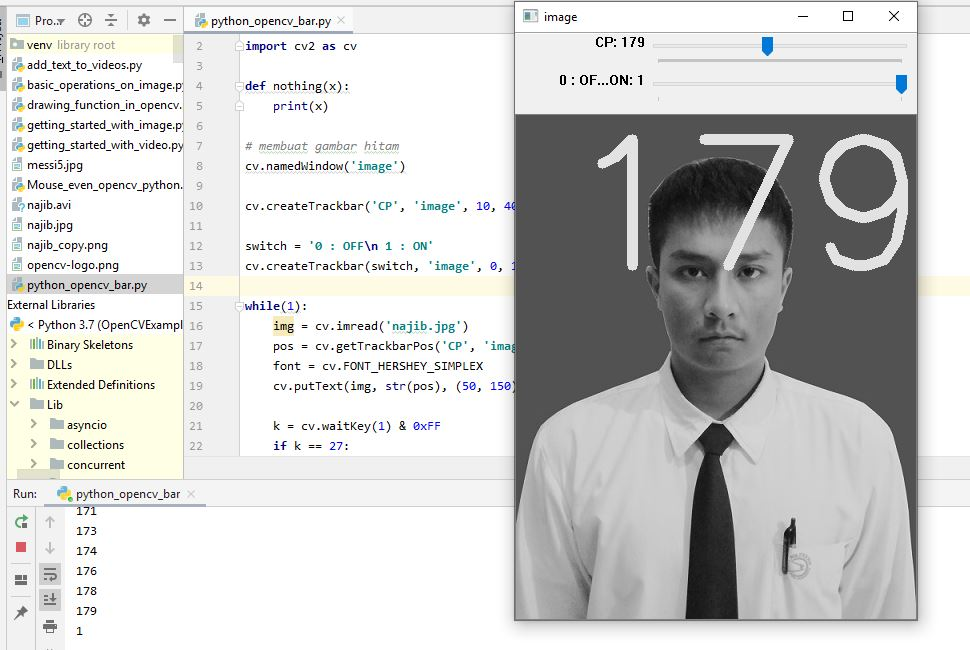
\includegraphics[scale=0.5]{figures/2,33,2.jpg}
\caption{Trackbar menampilkan text kontras}
\label{contoh}
\end{figure}



\newpage
\section{Object Detection dan Object Tracking menggunakan HSV Color Space}
\subsection{Membuat frame kosong}
\lstinputlisting{src/cv34.py}
\begin{enumerate}
	\item import numpy
	\item import cv
	\item membuat variable untuk menampilkan
	\item buat jendela atau frame baru dengan nama Tracking
	\item buat perulangan jika true maka akan melanjutkan perintah perulangan
	\item mengambil gambar dari file
	\item menampilkan gambar pada frame dengan nama frame
	\item membuat waitKey jika sama dengan 27 maka akan berakhir
	\item destroyAllWindows digunakan untuk menutup frame.
\end{enumerate}

\newpage
\begin{figure}[ht]
\centering
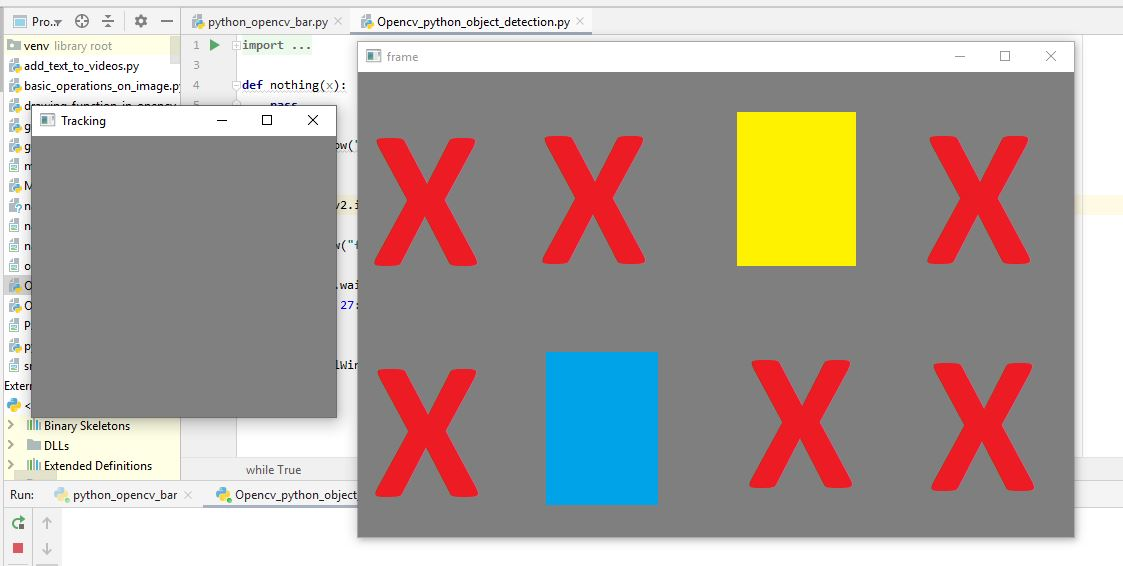
\includegraphics[scale=0.43]{figures/2,34.jpg}
\caption{Membuat frame kosong}
\label{contoh}
\end{figure}



\newpage
\subsection{Hsv color space}
\lstinputlisting{src/cv35.py}
\begin{enumerate}
	\item import numpy
	\item import cv
	\item membuat variable untuk menampilkan
	\item buat perulangan jika true maka akan melanjutkan perintah perulangan
	\item mengambil gambar dari file
	\item membuat variable dengan memanggil fungsi hsv
	\item membuat variable lb untuk menentukan angka pertama yaitu h kedua s dan ketiga v
	\item membuat variable ub untuk menentukan angka pertama yaitu h kedua s dan ketiga v
	\item variable mask di gunakan untuk menggabungkan hsv lb dan ub, mask juga membuat kontras warna menjadi hitam putih
	\item res digunakan untuk menggabungkan mask dan frame yang pertama
	\item menampilkan frame asli, frame mask, dan frame res
	\item membuat waitKey jika sama dengan 27 maka akan berakhir
	\item destroyAllWindows digunakan untuk menutup frame.
\end{enumerate}

\begin{figure}[ht]
\centering
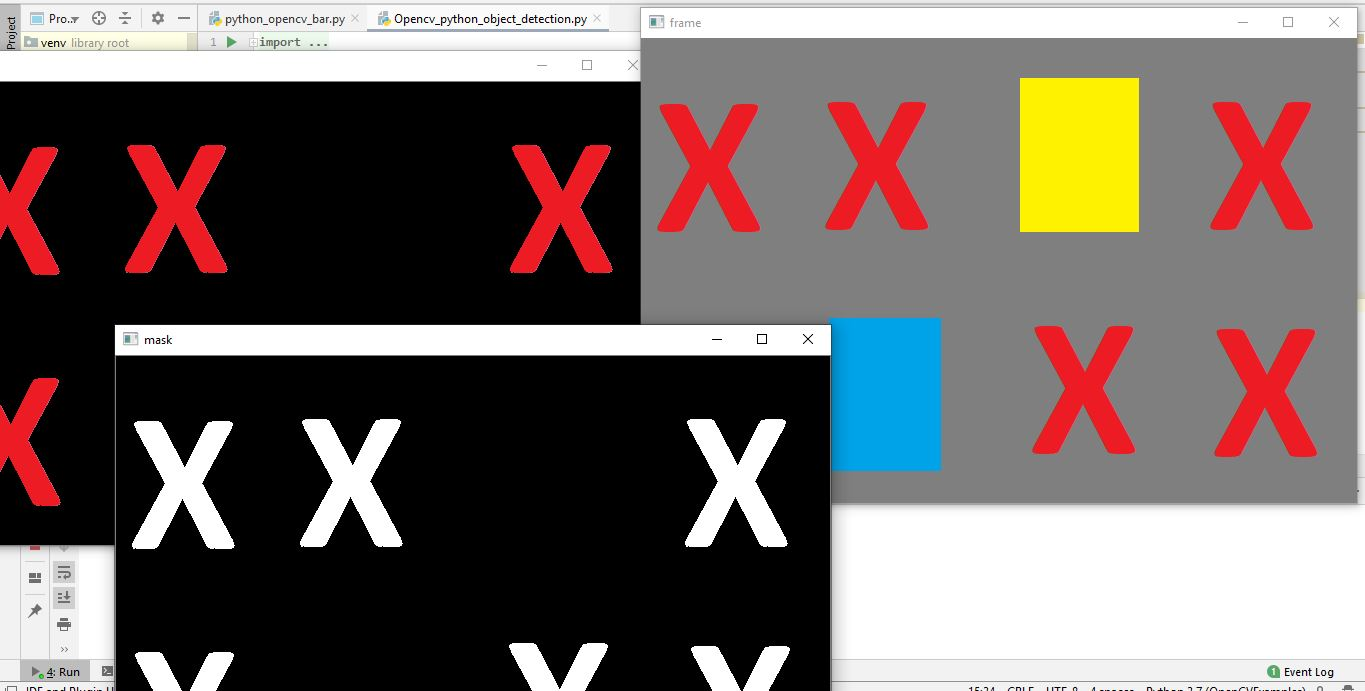
\includegraphics[scale=0.35]{figures/2,35.jpg}
\caption{Hsv color space}
\label{contoh}
\end{figure}



\newpage
\subsection{Hsv color space menggunakan Trackbar}
\lstinputlisting{src/cv36.py}
\begin{enumerate}
	\item import numpy
	\item import cv
	\item membuat variable untuk menampilkan
	\item membuat frame baru dengan nama Tracking
	\item membuat isi dari frame Tracking untuk menentukan kontras warna yang di inginkan sesuai hsv
	\item buat perulangan jika true maka akan melanjutkan perintah perulangan
	\item mengambil gambar dari file
	\item membuat variable dengan memanggil fungsi hsv, fungsi hsf digunakan untuk menampilkan warna tertentu saja jadi jika kita ingin menampilkan warna biru saja maka warna lain akan menjadi hitam bisa kita atur dengan mudah menggunakan traking tadi, jika sudah menemukan nomornya kita dapat masukan ke kede yang kita buat
	\item kemudian ambil data dari Tracking menggunakan getTrackbarPos
	\item membuat variable lb untuk menentukan angka pertama yaitu h kedua s dan ketiga v
	\item membuat variable ub untuk menentukan angka pertama yaitu h kedua s dan ketiga v
	\item variable mask di gunakan untuk menggabungkan hsv lb dan ub, mask juga membuat kontras warna menjadi hitam putih
	\item res digunakan untuk menggabungkan mask dan frame yang pertama
	\item menampilkan frame asli, frame mask, dan frame res
	\item membuat waitKey jika sama dengan 27 maka akan berakhir
	\item destroyAllWindows digunakan untuk menutup frame.
\end{enumerate}

\newpage
\begin{figure}[ht]
\centering
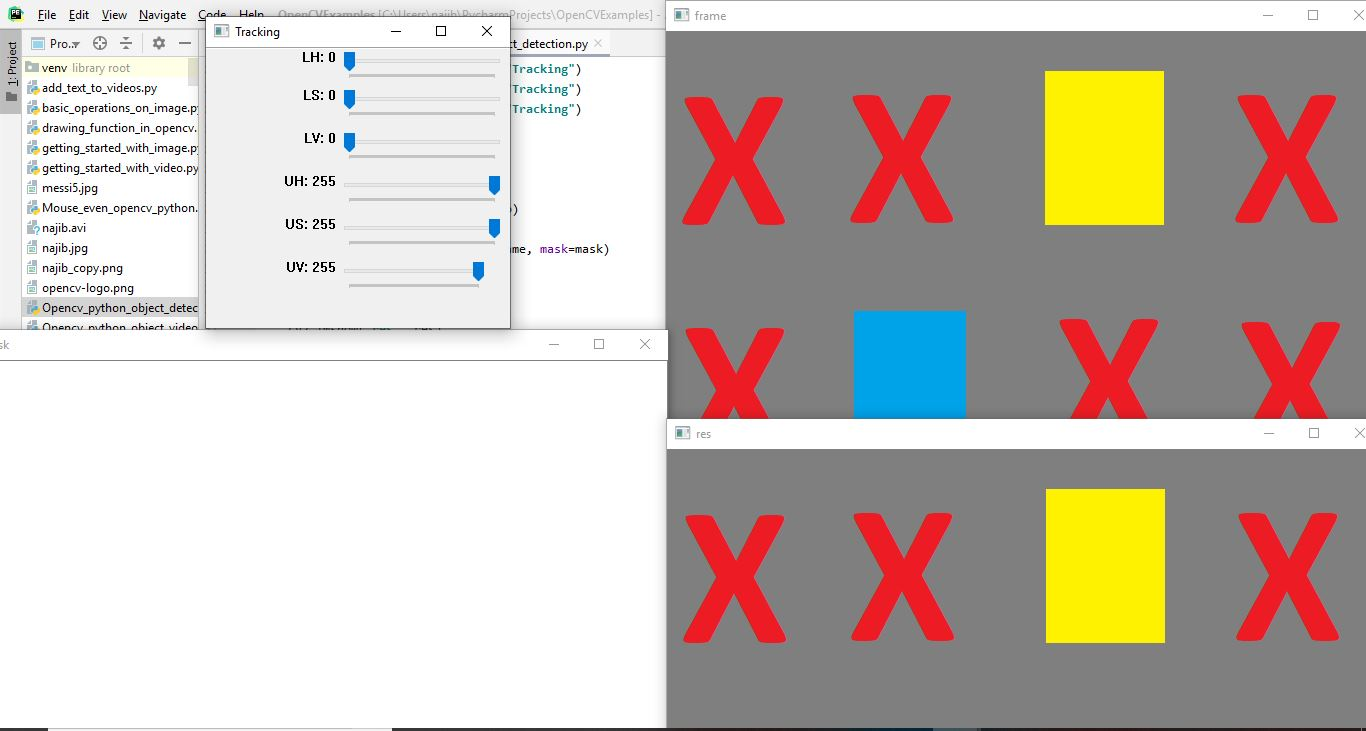
\includegraphics[scale=0.35]{figures/2,36.jpg}
\caption{Hsv color space menggunakan Trackbar}
\label{contoh}
\end{figure}

\begin{figure}[ht]
\centering
\includegraphics[scale=0.35]{figures/2,36,1.jpg}
\caption{Hsv color space menggunakan Trackbar}
\label{contoh}
\end{figure}

\newpage
\begin{figure}[ht]
\centering
\includegraphics[scale=0.35]{figures/2,36,2.jpg}
\caption{Hsv color space menggunakan Trackbar}
\label{contoh}
\end{figure}

\newpage
\begin{figure}[ht]
\centering
\includegraphics[scale=0.35]{figures/2,36,3.jpg}
\caption{Hsv color space menggunakan Trackbar}
\label{contoh}
\end{figure}



\newpage
\subsection{Menentukan kontras warna menggunakan Trackbar pada video}
\lstinputlisting{src/cv37.py}
\begin{enumerate}
	\item import numpy
	\item import cv
	\item membuat variable untuk menampilkan
	\item gunakan videocapture
	\item membuat frame baru dengan nama Tracking
	\item membuat isi dari frame Tracking untuk menentukan kontras warna yang di inginkan sesuai hsv
	\item buat perulangan jika true maka akan melanjutkan perintah perulangan
	\item membaca video
	\item membuat variable dengan memanggil fungsi hsv, fungsi hsf digunakan untuk menampilkan warna tertentu saja jadi jika kita ingin menampilkan warna biru saja maka warna lain akan menjadi hitam bisa kita atur dengan mudah menggunakan traking tadi, jika sudah menemukan nomornya kita dapat masukan ke kede yang kita buat
	\item kemudian ambil data dari Tracking menggunakan getTrackbarPos
	\item membuat variable lb untuk menentukan angka pertama yaitu h kedua s dan ketiga v
	\item membuat variable ub untuk menentukan angka pertama yaitu h kedua s dan ketiga v
	\item variable mask di gunakan untuk menggabungkan hsv lb dan ub, mask juga membuat kontras warna menjadi hitam putih
	\item res digunakan untuk menggabungkan mask dan frame yang pertama
	\item menampilkan frame asli, frame mask, dan frame res
	\item membuat waitKey jika sama dengan 27 maka akan berakhir
	\item destroyAllWindows digunakan untuk menutup frame.
\end{enumerate}

\newpage
\begin{figure}[ht]
\centering
\includegraphics[scale=0.35]{figures/2,37.jpg}
\caption{Menentukan kontras warna menggunakan Trackbar pada video}
\label{contoh}
\end{figure}



\newpage
\section{Image Thresholding}
\subsection{Membuat kontras warna menggunakan Binary}
\lstinputlisting{src/cv38.py}
\begin{enumerate}
	\item import cv2
	\item import numpy
	\item membaca gambar dengan kontras warna hitam putih
	\item membuat gambar dengan menggunakan event binary untuk menampilkan warna hitamnya 127 yang artinya setengan dari frame
	\item membuat frame image untuk menampilkan gambar
	\item membuat frame untuk gambar yang baru
	\item membuat waitKey supaya frame tidak langsung tertutup
	\item destroyAllWindows digunakan untuk menutup frame.
\end{enumerate}

\newpage
\begin{figure}[ht]
\centering
\includegraphics[scale=0.5]{figures/2,38.jpg}
\caption{Membuat kontras warna menggunakan Binary}
\label{contoh}
\end{figure}
Pada gambar ini menunjukan pada gambar terdapat warna apa saja dan menggunakan Binary warna jadi hanya terbagi menjadi 2 dan di tentukan ukurannya sesuai kebutuhan.




\newpage
\subsection{Membuat kontras warna menggunakan Binary Inv}
\lstinputlisting{src/cv39.py}
\begin{enumerate}
	\item import cv2
	\item import numpy
	\item membaca gambar dengan kontras warna hitam putih
	\item membuat gambar dengan menggunakan event binary untuk menampilkan warna hitamnya 127 yang artinya setengan dari frame
	\item membuat gambar dengan menggunakan event binary inv yaitu kebalikan dari binary
	\item membuat frame image untuk menampilkan gambar
	\item membuat frame untuk gambar yang baru th1
	\item membuat frame untuk gambar yang baru th2
	\item membuat waitKey supaya frame tidak langsung tertutup
	\item destroyAllWindows digunakan untuk menutup frame.
\end{enumerate}

\newpage
\begin{figure}[ht]
\centering
\includegraphics[scale=0.45]{figures/2,39.jpg}
\caption{Membuat kontras warna menggunakan Binary Inv}
\label{contoh}
\end{figure}
Pada gambar menunjukan perbedaan antara binary dan binary inv yaitu kebalikannya warna putihnya di sebelah kiri.




\newpage
\subsection{Membuat kontras warna menggunakan Trunc}
\lstinputlisting{src/cv40.py}
\begin{enumerate}
	\item import cv2
	\item import numpy
	\item membaca gambar dengan kontras warna hitam putih
	\item membuat gambar dengan menggunakan event binary untuk menampilkan warna hitamnya 127 yang artinya setengan dari frame
	\item membuat gambar dengan menggunakan event binary inv yaitu kebalikan dari binary
	\item membuat gambar dengan menggunakan event Trunc membuat kontras 
	\item membuat frame image untuk menampilkan gambar
	\item membuat frame untuk gambar yang baru th1
	\item membuat frame untuk gambar yang baru th2
	\item membuat frame untuk gambar yang baru th3
	\item membuat waitKey supaya frame tidak langsung tertutup
	\item destroyAllWindows digunakan untuk menutup frame.
\end{enumerate}

\newpage
\begin{figure}[ht]
\centering
\includegraphics[scale=0.42]{figures/2,40.jpg}
\caption{Membuat kontras warna menggunakan Trunc}
\label{contoh}
\end{figure}
Pada gambar menunjukan event Trunc mengubah gambar menjadi warna terrendahnya berada di tengah




\newpage
\subsection{Membuat kontras warna menggunakan Tozero}
\lstinputlisting{src/cv41.py}
\begin{enumerate}
	\item import cv2
	\item import numpy
	\item membaca gambar dengan kontras warna hitam putih
	\item membuat gambar dengan menggunakan event binary untuk menampilkan warna hitamnya 127 yang artinya setengan dari frame
	\item membuat gambar dengan menggunakan event binary inv yaitu kebalikan dari binary
	\item membuat gambar dengan menggunakan event Trunc membuat kontras 
	\item membuat gambar dengan menggunakan event Tozero berguna untuk memperjelas warna tergelap
	\item membuat frame image untuk menampilkan gambar
	\item membuat frame untuk gambar yang baru th1
	\item membuat frame untuk gambar yang baru th2
	\item membuat frame untuk gambar yang baru th3
	\item membaut frame untuk gambar yang baru th4
	\item membuat waitKey supaya frame tidak langsung tertutup
	\item destroyAllWindows digunakan untuk menutup frame.
\end{enumerate}

\newpage
\begin{figure}[ht]
\centering
\includegraphics[scale=0.42]{figures/2,41.jpg}
\caption{Membuat kontras warna menggunakan Tozero}
\label{contoh}
\end{figure}
pada gambar menampilkan perbedaan antara Tozero dan yang lainnya Tozero menunjukan menampilkan kontras tergela dan yeng sebelahnya tetap sesuai gambar.



\newpage
\subsection{Membuat kontras warna menggunakan Tozero Inv}
\lstinputlisting{src/cv42.py}
\begin{enumerate}
	\item import cv2
	\item import numpy
	\item membaca gambar dengan kontras warna hitam putih
	\item membuat gambar dengan menggunakan event binary untuk menampilkan warna hitamnya 127 yang artinya setengan dari frame
	\item membuat gambar dengan menggunakan event binary inv yaitu kebalikan dari binary
	\item membuat gambar dengan menggunakan event Trunc membuat kontras 
	\item membuat gambar dengan menggunakan event Tozero berguna untuk memperjelas warna tergelap
	\item membuat gambar dengan menggunakan event Tozero Inv kebalika dari tonzero
	\item membuat frame image untuk menampilkan gambar
	\item membuat frame untuk gambar yang baru th1
	\item membuat frame untuk gambar yang baru th2
	\item membuat frame untuk gambar yang baru th3
	\item membaut frame untuk gambar yang baru th4
	\item membaut frame untuk gambar yang baru th5
	\item membuat waitKey supaya frame tidak langsung tertutup
	\item destroyAllWindows digunakan untuk menutup frame.
\end{enumerate}

\begin{figure}[ht]
\centering
\includegraphics[scale=0.42]{figures/2,42.jpg}
\caption{Membuat kontras warna menggunakan Tozero Inv}
\label{contoh}
\end{figure}
Tonzero Inv merupakan kebalikan dari tonzero menmpilkan kontras tergelap di sebelah kanan




\newpage
\section{Adative Thresholding}
\subsection{Mengubah warna gambar menggunakan Binary}
\lstinputlisting{src/cv43.py}
\begin{enumerate}
	\item import cv2
	\item import numpy
	\item membaca gambar dengan kontras warna hitam putih
	\item membuat gambar dengan menggunakan event binary untuk menampilkan warna hitamnya 127 yang artinya setengan dari frame
	\item membuat frame image untuk menampilkan gambar
	\item membuat frame untuk gambar yang baru
	\item membuat waitKey supaya frame tidak langsung tertutup
	\item destroyAllWindows digunakan untuk menutup frame.
\end{enumerate}

\newpage
\begin{figure}[ht]
\centering
\includegraphics[scale=0.47]{figures/2,43.jpg}
\caption{Mengubah warna gambar menggunakan Binary}
\label{contoh}
\end{figure}
Pada sebuah foto warna yang mendekati dengan putih akan berubah menjadi putih dan sebaliknya jika warna mendekati dengan warna hitam maka warna akan berubah menjadi warna hitam.




\newpage
\subsection{Menggunakan Adaptive Thresh Mean}
\lstinputlisting{src/cv44.py}
\begin{enumerate}
	\item import cv2
	\item import numpy
	\item membaca gambar dengan kontras warna hitam putih
	\item membuat gambar dengan menggunakan event binary untuk menampilkan warna hitamnya 127 yang artinya setengan dari frame
	\item menggunakan event Adaptive Thresh mean
	\item membuat frame image untuk menampilkan gambar
	\item membuat frame untuk gambar yang baru
	\item membuat frame untuk adaptive
	\item membuat waitKey supaya frame tidak langsung tertutup
	\item destroyAllWindows digunakan untuk menutup frame.
\end{enumerate}

\newpage
\begin{figure}[ht]
\centering
\includegraphics[scale=0.38]{figures/2,44.jpg}
\caption{Menggunakan Adaptive Thresh Mean}
\label{contoh}
\end{figure}
pada gambar gambar menyesuaikan kontras hitamnya saja yang tidak ada kontras maka akan berubah menjadi putih







\newpage
\subsection{Menggunakan Adaptive Thresh Gaussian}
\lstinputlisting{src/cv45.py}
\begin{enumerate}
	\item import cv2
	\item import numpy
	\item membaca gambar dengan kontras warna hitam putih
	\item membuat gambar dengan menggunakan event binary untuk menampilkan warna hitamnya 127 yang artinya setengan dari frame
	\item menggunakan event Adaptive Thresh mean
	\item menggunakan event Adaptive Thresh Gaussian
	\item membuat frame image untuk menampilkan gambar
	\item membuat frame untuk gambar yang baru
	\item membuat frame untuk adaptive mean
	\item membuat frame untuk adaptive gaussian
	\item membuat waitKey supaya frame tidak langsung tertutup
	\item destroyAllWindows digunakan untuk menutup frame.
\end{enumerate}

\newpage
\begin{figure}[ht]
\centering
\includegraphics[scale=0.35]{figures/2,45.jpg}
\caption{Menggunakan Adaptive Thresh Gaussian}
\label{contoh}
\end{figure}
Event adaptive Thresh Gaussian terlihat lebih smooth dibangdingkan dengan event Adaptive Thresh Mean.




\newpage
\section{Menggunakan Matplotlip pada OpenCV}
\subsection{Installasi Matplotlib}
Menginstall Matplotlib pada pycharp yang perlu kita lakukan masuk pada menu settings kemudian masuk pada menu Project Interpreter lalu klik tambah untuk menambahkan library yang ada pada project kita.
\begin{figure}[ht]
\centering
\includegraphics[scale=0.45]{figures/2,46.jpg}
\caption{Installasi matplotlib}
\label{contoh}
\end{figure}

\newpage
kemudian cari pada pencarian yaitu matplotlip jika sudah menemukan kita hanya perlu klik laku insatall package.
\begin{figure}[ht]
\centering
\includegraphics[scale=0.45]{figures/2,46,1.jpg}
\caption{Installasi matplotlib}
\label{contoh}
\end{figure}

\newpage
jika matplotlib sudah terinstall maka akan di tampilkan pada halaman daftar library yang di gunakan pada project seperti pada gambar.
\begin{figure}[ht]
\centering
\includegraphics[scale=0.45]{figures/2,46,2.jpg}
\caption{Installasi matplotlib}
\label{contoh}
\end{figure}





\newpage
\subsection{Menampilkan gambar menggunakan matplotlib}
\lstinputlisting{src/cv46.py}
\begin{enumerate}
	\item import cv
	\item import matplotlib
	\item mengambil gambar pada file menggunakan imread dengan kontras -1 yang artinya sesuai asli gambar
	\item membuat frame dengan nama image
	\item menampilkan gambar
	\item menampilkan gambar sesuai matplotlib
	\item membuat waitKey supaya frame tidak langsung tertutup
	\item destroyAllWindows digunakan untuk menutup frame.
\end{enumerate}

\newpage
\begin{figure}[ht]
\centering
\includegraphics[scale=0.42]{figures/2,46,3.jpg}
\caption{Menampilkan gambar menggunakan matplotlib}
\label{contoh}
\end{figure}
pada gambar yang di tampilkan menggunakan plot pada framenya terdapat berbagai tools dapat di zoom, mengubah ukuran gambar yang di tampilkan sesuai yang di inginkan dan dapat belihat titik x dan y





\newpage
\subsection{Mengubah warna yang ditampilkan matplotlib}
\lstinputlisting{src/cv47.py}
\begin{enumerate}
	\item import cv
	\item import matplotlib
	\item mengambil gambar pada file menggunakan imread dengan kontras -1 yang artinya sesuai asli gambar
	\item membuat frame dengan nama image
	\item membuat tampilan yang di tampilkan menggunakan matplotlib warnanya sesuai aslinya
	\item menampilkan gambar
	\item menampilkan gambar sesuai matplotlib
	\item membuat waitKey supaya frame tidak langsung tertutup
	\item destroyAllWindows digunakan untuk menutup frame.
\end{enumerate}

\newpage
\begin{figure}[ht]
\centering
\includegraphics[scale=0.42]{figures/2,47.jpg}
\caption{Mengubah warna yang ditampilkan matplotlib}
\label{contoh}
\end{figure}
Pada gambar sebelumnya gambar yang di tampilkan menggunakan matplotlib berwarna birun, menggunakan cvtcolor mwmbuat yang di tampilkan sesuai dengan aslinya

\newpage
untuk mengubah ukuran kita dapat mengubahnya seperti pada gambar sesuai yang di inginkan
\begin{figure}[ht]
\centering
\includegraphics[scale=0.4]{figures/2,47,1.jpg}
\caption{Mengubah warna yang ditampilkan matplotlib}
\label{contoh}
\end{figure}





\newpage
\subsection{Menghilangkan koordinat x dan y pada tampilan matplotlib}
\lstinputlisting{src/cv48.py}
\begin{enumerate}
	\item import cv
	\item import matplotlib
	\item mengambil gambar pada file menggunakan imread dengan kontras -1 yang artinya sesuai asli gambar
	\item membuat frame dengan nama image
	\item membuat tampilan yang di tampilkan menggunakan matplotlib warnanya sesuai aslinya
	\item menampilkan gambar
	\gunakan xticks dan yticks untuk menghilangkan nomor nomor koordinat x dan y yang di tampilkan oleh matplotlib
	\item menampilkan gambar sesuai matplotlib
	\item membuat waitKey supaya frame tidak langsung tertutup
	\item destroyAllWindows digunakan untuk menutup frame.
\end{enumerate}

\newpage
\begin{figure}[ht]
\centering
\includegraphics[scale=0.4]{figures/2,48.jpg}
\caption{Menghilangkan koordinat x dan y pada tampilan matplotlib}
\label{contoh}
\end{figure}
Pada gambar sebelumya gambar yang di tampilkan oleh matplotlib terdapat nomor nomor koordinat x dan y, menggunakan xticks dan yticks koordinat tersebut di hilangkan






\newpage
\subsection{Menggabungkan frame menjadi satu frame}
\lstinputlisting{src/cv49.py}
\begin{enumerate}
	\item import cv2
	\item import numpy
	\item import matplotlib
	\item membaca gambar dengan kontras warna hitam putih
	\item membuat gambar dengan menggunakan event binary untuk menampilkan warna hitamnya 127 yang artinya setengan dari frame
	\item membuat gambar dengan menggunakan event binary inv yaitu kebalikan dari binary
	\item membuat gambar dengan menggunakan event Trunc membuat kontras 
	\item membuat gambar dengan menggunakan event Tozero berguna untuk memperjelas warna tergelap
	\item membuat gambar dengan menggunakan event Tozero Inv kebalika dari tonzero
	\item membuat judul pada setiap gambar di satu frame
	\item memetakan gambar gambar yang akan di tampilkan
	\item menampilkan 6 gambar pada satu frame
	\item menampilkan gambar dengan 2 kolom 3 baris menampilkan gambar sesuai urutan gambar
	\item menampilkan judul sesuai urutan judul
	\item tidak menampilkan koordinat matplotlib
	\item menampilkan gambar
\end{enumerate}

\begin{figure}[ht]
\centering
\includegraphics[scale=0.5]{figures/2,49.jpg}
\caption{Menggabungkan frame menjadi satu frame}
\label{contoh}
\end{figure}




\newpage
\section{Morphologikan Transformations}
\subsection{Menggunakan imread grayscale}
\lstinputlisting{src/cv50.py}
\begin{enumerate}
	\item import cv2
	\item import numpy
	\item import matplotlib
	\item memanggil gambar lalu gambar diberi event Grayscale untuk merubah gambar menjadi hitam putih
	\item membuat judul gambar
	\item memanggil gambar
	\item menampilkan 1 gambar pada satu frame
	\item menampilkan gambar dengan 1 kolom 1 baris menampilkan gambar sesuai urutan gambar
	\item menampilkan judul sesuai urutan judul
	\item tidak menampilkan koordinat matplotlib
	\item menampilkan gambar
\end{enumerate}

\newpage
\begin{figure}[ht]
\centering
\includegraphics[scale=0.6]{figures/2,50.jpg}
\caption{Menggunakan imread grayscale}
\label{contoh}
\end{figure}
Gambar berubah menjadi hitam putih






\newpage
\subsection{Menggunakan Thresh Binary Inv}
\lstinputlisting{src/cv51.py}
\begin{enumerate}
	\item import cv2
	\item import numpy
	\item import matplotlib
	\item memanggil gambar lalu gambar diberi event Grayscale untuk merubah gambar menjadi hitam putih
	\item mengambil gambar yang sama tetapi menggunakan event Thresh Binary Inv, menghitamkan warna putih dan memutihkan yang berwarna
	\item membuat judul gambar
	\item memanggil gambar
	\item menampilkan 2 gambar pada satu frame
	\item menampilkan gambar dengan 1 kolom 2 baris menampilkan gambar sesuai urutan gambar
	\item menampilkan judul sesuai urutan judul
	\item tidak menampilkan koordinat matplotlib
	\item menampilkan gambar
\end{enumerate}

\newpage
\begin{figure}[ht]
\centering
\includegraphics[scale=0.6]{figures/2,51.jpg}
\caption{Menggunakan Thresh Binary Inv}
\label{contoh}
\end{figure}








\newpage
\subsection{Menggunakan Dilate}
\lstinputlisting{src/cv52.py}
\begin{enumerate}
	\item import cv2
	\item import numpy
	\item import matplotlib
	\item memanggil gambar lalu gambar diberi event Grayscale untuk merubah gambar menjadi hitam putih
	\item mengambil gambar yang sama tetapi menggunakan event Thresh Binary Inv, menghitamkan warna putih dan memutihkan yang berwarna
	\item membuat karnal menggunakan numpy dengan type warna uint8
	\item dilation di gunakan untuk membuat gambar lebih terlihat smooth, menghilangkan bintik bintik kecil
	\item membuat judul gambar
	\item memanggil gambar
	\item menampilkan 3 gambar pada satu frame
	\item menampilkan gambar dengan 1 kolom 3 baris menampilkan gambar sesuai urutan gambar
	\item menampilkan judul sesuai urutan judul
	\item tidak menampilkan koordinat matplotlib
	\item menampilkan gambar
\end{enumerate}

\begin{figure}[ht]
\centering
\includegraphics[scale=0.6]{figures/2,52.jpg}
\caption{Menggunakan Dilate}
\label{contoh}
\end{figure}







\newpage
\subsection{Mengubah ukuran karnal}
\lstinputlisting{src/cv53.py}
\begin{enumerate}
	\item import cv2
	\item import numpy
	\item import matplotlib
	\item memanggil gambar lalu gambar diberi event Grayscale untuk merubah gambar menjadi hitam putih
	\item mengambil gambar yang sama tetapi menggunakan event Thresh Binary Inv, menghitamkan warna putih dan memutihkan yang berwarna
	\item membuat karnal menggunakan numpy dengan type warna uint8, semakin besar ukuran karnal semakin smooth gambar yang di hasilkan tetap sesuai kebutuhan penggunaan
	\item dilation di gunakan untuk membuat gambar lebih terlihat smooth, menghilangkan bintik bintik kecil
	\item membuat judul gambar
	\item memanggil gambar
	\item menampilkan 4 gambar pada satu frame
	\item menampilkan gambar dengan 2 kolom 2 baris menampilkan gambar sesuai urutan gambar
	\item menampilkan judul sesuai urutan judul
	\item tidak menampilkan koordinat matplotlib
	\item menampilkan gambar
\end{enumerate}

\begin{figure}[ht]
\centering
\includegraphics[scale=0.6]{figures/2,53.jpg}
\caption{Mengubah ukuran karnal}
\label{contoh}
\end{figure}







\newpage
\subsection{Menggunakan Erode}
\lstinputlisting{src/cv54.py}
\begin{enumerate}
	\item import cv2
	\item import numpy
	\item import matplotlib
	\item memanggil gambar lalu gambar diberi event Grayscale untuk merubah gambar menjadi hitam putih
	\item mengambil gambar yang sama tetapi menggunakan event Thresh Binary Inv, menghitamkan warna putih dan memutihkan yang berwarna
	\item membuat karnal menggunakan numpy dengan type warna uint8, semakin besar ukuran karnal semakin smooth gambar yang di hasilkan tetap sesuai kebutuhan penggunaan
	\item dilation di gunakan untuk membuat gambar lebih terlihat smooth, menghilangkan bintik bintik kecil
	\item erosion atau yang pada event di sebut erode berguna untuk sedikit warna yang mendekati putih akan berubah menjadi hitam
	\item membuat judul gambar
	\item memanggil gambar
	\item menampilkan 5 gambar pada satu frame
	\item menampilkan gambar dengan 2 kolom 3 baris menampilkan gambar sesuai urutan gambar
	\item menampilkan judul sesuai urutan judul
	\item tidak menampilkan koordinat matplotlib
	\item menampilkan gambar
\end{enumerate}

\begin{figure}[ht]
\centering
\includegraphics[scale=0.6]{figures/2,54.jpg}
\caption{Menggunakan Erode}
\label{contoh}
\end{figure}







\newpage
\subsection{Menggunakan MorphologyEx Open}
\lstinputlisting{src/cv55.py}
\begin{enumerate}
	\item import cv2
	\item import numpy
	\item import matplotlib
	\item memanggil gambar lalu gambar diberi event Grayscale untuk merubah gambar menjadi hitam putih
	\item mengambil gambar yang sama tetapi menggunakan event Thresh Binary Inv, menghitamkan warna putih dan memutihkan yang berwarna
	\item membuat karnal menggunakan numpy dengan type warna uint8, semakin besar ukuran karnal semakin smooth gambar yang di hasilkan tetap sesuai kebutuhan penggunaan
	\item dilation di gunakan untuk membuat gambar lebih terlihat smooth, menghilangkan bintik bintik kecil
	\item erosion atau yang pada event di sebut erode berguna untuk sedikit warna yang mendekati putih akan berubah menjadi hitam
	\item morphology hampirsama dengan Thresh Binary Inv
	\item membuat judul gambar
	\item memanggil gambar
	\item menampilkan 6 gambar pada satu frame
	\item menampilkan gambar dengan 2 kolom 3 baris menampilkan gambar sesuai urutan gambar
	\item menampilkan judul sesuai urutan judul
	\item tidak menampilkan koordinat matplotlib
	\item menampilkan gambar
\end{enumerate}

\begin{figure}[ht]
\centering
\includegraphics[scale=0.6]{figures/2,55.jpg}
\caption{Menggunakan MorphologyEx Open}
\label{contoh}
\end{figure}







\newpage
\subsection{Menggunakan MorphologyEx Close}
\lstinputlisting{src/cv56.py}
\begin{enumerate}
	\item import cv2
	\item import numpy
	\item import matplotlib
	\item memanggil gambar lalu gambar diberi event Grayscale untuk merubah gambar menjadi hitam putih
	\item mengambil gambar yang sama tetapi menggunakan event Thresh Binary Inv, menghitamkan warna putih dan memutihkan yang berwarna
	\item membuat karnal menggunakan numpy dengan type warna uint8, semakin besar ukuran karnal semakin smooth gambar yang di hasilkan tetap sesuai kebutuhan penggunaan
	\item dilation di gunakan untuk membuat gambar lebih terlihat smooth, menghilangkan bintik bintik kecil
	\item erosion atau yang pada event di sebut erode berguna untuk sedikit warna yang mendekati putih akan berubah menjadi hitam
	\item morphology open hampirsama dengan Thresh Binary Inv
	\item morphology close lebis smooth dibanding open
	\item membuat judul gambar
	\item memanggil gambar
	\item menampilkan 7 gambar pada satu frame
	\item menampilkan gambar dengan 2 kolom 4 baris menampilkan gambar sesuai urutan gambar
	\item menampilkan judul sesuai urutan judul
	\item tidak menampilkan koordinat matplotlib
	\item menampilkan gambar
\end{enumerate}

\begin{figure}[ht]
\centering
\includegraphics[scale=0.6]{figures/2,56.jpg}
\caption{Menggunakan MorphologyEx Close}
\label{contoh}
\end{figure}






\newpage
\subsection{Menggunakan MorphologyEx Gradient}
\lstinputlisting{src/cv57.py}
\begin{enumerate}
	\item import cv2
	\item import numpy
	\item import matplotlib
	\item memanggil gambar lalu gambar diberi event Grayscale untuk merubah gambar menjadi hitam putih
	\item mengambil gambar yang sama tetapi menggunakan event Thresh Binary Inv, menghitamkan warna putih dan memutihkan yang berwarna
	\item membuat karnal menggunakan numpy dengan type warna uint8, semakin besar ukuran karnal semakin smooth gambar yang di hasilkan tetap sesuai kebutuhan penggunaan
	\item dilation di gunakan untuk membuat gambar lebih terlihat smooth, menghilangkan bintik bintik kecil
	\item erosion atau yang pada event di sebut erode berguna untuk sedikit warna yang mendekati putih akan berubah menjadi hitam
	\item morphology open hampirsama dengan Thresh Binary Inv
	\item morphology close lebis smooth dibanding open
	\item morphology gradient event ini mengambil warna luarnya saja warna dalamnya di ubah menjadi hitam
	\item membuat judul gambar
	\item memanggil gambar
	\item menampilkan 8 gambar pada satu frame
	\item menampilkan gambar dengan 2 kolom 4 baris menampilkan gambar sesuai urutan gambar
	\item menampilkan judul sesuai urutan judul
	\item tidak menampilkan koordinat matplotlib
	\item menampilkan gambar
\end{enumerate}

\begin{figure}[ht]
\centering
\includegraphics[scale=0.52]{figures/2,57.jpg}
\caption{Menggunakan MorphologyEx Gradient}
\label{contoh}
\end{figure}






\newpage
\subsection{Menggunakan MorphologyEx Tophat}
\lstinputlisting{src/cv58.py}
\begin{enumerate}
	\item import cv2
	\item import numpy
	\item import matplotlib
	\item memanggil gambar lalu gambar diberi event Grayscale untuk merubah gambar menjadi hitam putih
	\item mengambil gambar yang sama tetapi menggunakan event Thresh Binary Inv, menghitamkan warna putih dan memutihkan yang berwarna
	\item membuat karnal menggunakan numpy dengan type warna uint8, semakin besar ukuran karnal semakin smooth gambar yang di hasilkan tetap sesuai kebutuhan penggunaan
	\item dilation di gunakan untuk membuat gambar lebih terlihat smooth, menghilangkan bintik bintik kecil
	\item erosion atau yang pada event di sebut erode berguna untuk sedikit warna yang mendekati putih akan berubah menjadi hitam
	\item morphology open hampirsama dengan Thresh Binary Inv
	\item morphology close lebis smooth dibanding open
	\item morphology gradient event ini mengambil warna luarnya saja warna dalamnya di ubah menjadi hitam
	\item Tophat menampilkan warna tertentu
	\item membuat judul gambar
	\item memanggil gambar
	\item menampilkan 8 gambar pada satu frame
	\item menampilkan gambar dengan 2 kolom 4 baris menampilkan gambar sesuai urutan gambar
	\item menampilkan judul sesuai urutan judul
	\item tidak menampilkan koordinat matplotlib
	\item menampilkan gambar
\end{enumerate}

\begin{figure}[ht]
\centering
\includegraphics[scale=0.5]{figures/2,58.jpg}
\caption{Menggunakan MorphologyEx Tophat}
\label{contoh}
\end{figure}







\newpage
\section{Smoothing Images}
\subsection{Menggunakan Filter 2D}
\lstinputlisting{src/cv59.py}
\begin{enumerate}
	\item import cv2
	\item import numpy
	\item import matplotlib
	\item mengambil gambar dari file
	\item pada gambar yang di ambil digunakan kontras warna bgr blue, green, read
	\item buat karnel numpy yang berisi matriks per 25
	\item menggunakan event filter 2D
	\item membuat judul gambar
	\item memanggil gambar
	\item menampilkan 2 gambar pada satu frame
	\item menampilkan gambar dengan 1 kolom 2 baris menampilkan gambar sesuai urutan gambar
	\item menampilkan judul sesuai urutan judul
	\item tidak menampilkan koordinat matplotlib
	\item menampilkan gambar
\end{enumerate}

\begin{figure}[ht]
\centering
\includegraphics[scale=0.6]{figures/2,59.jpg}
\caption{Menggunakan Filter 2D}
\label{contoh}
\end{figure}







\newpage
\subsection{Menggunakan Event Blur}
\lstinputlisting{src/cv60.py}
\begin{enumerate}
	\item import cv2
	\item import numpy
	\item import matplotlib
	\item mengambil gambar dari file
	\item pada gambar yang di ambil digunakan kontras warna bgr blue, green, read
	\item buat karnel numpy yang berisi matriks per 25
	\item menggunakan event filter 2D
	\item menggunakan event blur
	\item membuat judul gambar
	\item memanggil gambar
	\item menampilkan 3 gambar pada satu frame
	\item menampilkan gambar dengan 1 kolom 3 baris menampilkan gambar sesuai urutan gambar
	\item menampilkan judul sesuai urutan judul
	\item tidak menampilkan koordinat matplotlib
	\item menampilkan gambar
\end{enumerate}

\begin{figure}[ht]
\centering
\includegraphics[scale=0.35]{figures/2,60.jpg}
\caption{Menggunakan Event Blur}
\label{contoh}
\end{figure}







\newpage
\subsection{Menggunakan Event Gaussian Blur}
\lstinputlisting{src/cv61.py}
\begin{enumerate}
	\item import cv2
	\item import numpy
	\item import matplotlib
	\item mengambil gambar dari file
	\item pada gambar yang di ambil digunakan kontras warna bgr blue, green, read
	\item buat karnel numpy yang berisi matriks per 25
	\item menggunakan event filter 2D
	\item menggunakan event blur
	\item menggunakan event Gaussian Blur event ini tidak terlalu ngeblur di banding event blur
	\item membuat judul gambar
	\item memanggil gambar
	\item menampilkan 4 gambar pada satu frame
	\item menampilkan gambar dengan 2 kolom 2 baris menampilkan gambar sesuai urutan gambar
	\item menampilkan judul sesuai urutan judul
	\item tidak menampilkan koordinat matplotlib
	\item menampilkan gambar
\end{enumerate}

\begin{figure}[ht]
\centering
\includegraphics[scale=0.5]{figures/2,61.jpg}
\caption{Menggunakan Event Gaussian Blur}
\label{contoh}
\end{figure}







\newpage
\subsection{Menggunakan Event Median Blur}
\lstinputlisting{src/cv62.py}
\begin{enumerate}
	\item import cv2
	\item import numpy
	\item import matplotlib
	\item mengambil gambar dari file
	\item pada gambar yang di ambil digunakan kontras warna bgr blue, green, read
	\item buat karnel numpy yang berisi matriks per 25
	\item menggunakan event filter 2D
	\item menggunakan event blur
	\item menggunakan event Gaussian Blur event ini tidak terlalu ngeblur di banding event blur
	\item menggunakan event median blur
	\item membuat judul gambar
	\item memanggil gambar
	\item menampilkan 5 gambar pada satu frame
	\item menampilkan gambar dengan 2 kolom 3 baris menampilkan gambar sesuai urutan gambar
	\item menampilkan judul sesuai urutan judul
	\item tidak menampilkan koordinat matplotlib
	\item menampilkan gambar
\end{enumerate}

\begin{figure}[ht]
\centering
\includegraphics[scale=0.6]{figures/2,62.jpg}
\caption{Menggunakan Event Median Blur}
\label{contoh}
\end{figure}







\newpage
\subsection{Menggunakan Event BilateralFilter}
\lstinputlisting{src/cv63.py}
\begin{enumerate}
	\item import cv2
	\item import numpy
	\item import matplotlib
	\item mengambil gambar dari file
	\item pada gambar yang di ambil digunakan kontras warna bgr blue, green, read
	\item buat karnel numpy yang berisi matriks per 25
	\item menggunakan event filter 2D
	\item menggunakan event blur
	\item menggunakan event Gaussian Blur event ini tidak terlalu ngeblur di banding event blur
	\item menggunakan event median blur
	\item menggunakan event Bilateral Filter
	\item membuat judul gambar
	\item memanggil gambar
	\item menampilkan 5 gambar pada satu frame
	\item menampilkan gambar dengan 2 kolom 3 baris menampilkan gambar sesuai urutan gambar
	\item menampilkan judul sesuai urutan judul
	\item tidak menampilkan koordinat matplotlib
	\item menampilkan gambar
\end{enumerate}

\begin{figure}[ht]
\centering
\includegraphics[scale=0.32]{figures/2,63.jpg}
\caption{Menggunakan Event BilateralFilter}
\label{contoh}
\end{figure}






\newpage
\section{Image Gradients}
\subsection{Menggunakan Event Laplacian}
\lstinputlisting{src/cv64.py}
\begin{enumerate}
	\item import cv2
	\item import numpy
	\item import matplotlib
	\item mengambil gambar dari file
	\item menggunakan event laplacian
	\item menggunakan numpay absolute
	\item membuat judul gambar
	\item memanggil gambar
	\item menampilkan 2 gambar pada satu frame
	\item menampilkan gambar dengan 1 kolom 2 baris menampilkan gambar sesuai urutan gambar
	\item menampilkan judul sesuai urutan judul
	\item tidak menampilkan koordinat matplotlib
	\item menampilkan gambar
\end{enumerate}

\newpage
\begin{figure}[ht]
\centering
\includegraphics[scale=0.6]{figures/2,64.jpg}
\caption{Menggunakan Event Laplacian}
\label{contoh}
\end{figure}






\newpage
\subsection{Menggunakan Event Laplacian menggunakan Size}
\lstinputlisting{src/cv65.py}
\begin{enumerate}
	\item import cv2
	\item import numpy
	\item import matplotlib
	\item mengambil gambar dari file
	\item menggunakan event laplacian gunakan size untuk lebih memperjelas kegunaan laplacian, setelah di tambahkan size gambar berubah menjadi lebih jelas
	\item menggunakan numpay absolute
	\item membuat judul gambar
	\item memanggil gambar
	\item menampilkan 2 gambar pada satu frame
	\item menampilkan gambar dengan 1 kolom 2 baris menampilkan gambar sesuai urutan gambar
	\item menampilkan judul sesuai urutan judul
	\item tidak menampilkan koordinat matplotlib
	\item menampilkan gambar
\end{enumerate}

\newpage
\begin{figure}[ht]
\centering
\includegraphics[scale=0.6]{figures/2,65.jpg}
\caption{Menggunakan Event Laplacian menggunakan Size}
\label{contoh}
\end{figure}








\newpage
\subsection{Menggunakan Event Sobel X}
\lstinputlisting{src/cv66.py}
\begin{enumerate}
	\item import cv2
	\item import numpy
	\item import matplotlib
	\item mengambil gambar dari file
	\item menggunakan event laplacian gunakan size untuk lebih memperjelas kegunaan laplacian, setelah di tambahkan size gambar berubah menjadi lebih jelas
	\item menggunakan numpay absolute
	\item menggunakan event sobel
	\item menggunakan matriks sobelx agar mengarah ke kanan karana mengarah ke x
	\item membuat judul gambar
	\item memanggil gambar
	\item menampilkan 3 gambar pada satu frame
	\item menampilkan gambar dengan 2 kolom 2 baris menampilkan gambar sesuai urutan gambar
	\item menampilkan judul sesuai urutan judul
	\item tidak menampilkan koordinat matplotlib
	\item menampilkan gambar
\end{enumerate}

\begin{figure}[ht]
\centering
\includegraphics[scale=0.5]{figures/2,66.jpg}
\caption{Menggunakan Event Sobel X}
\label{contoh}
\end{figure}







\newpage
\subsection{Menggunakan Event Sobel Y}
\lstinputlisting{src/cv67.py}
\begin{enumerate}
	\item import cv2
	\item import numpy
	\item import matplotlib
	\item mengambil gambar dari file
	\item menggunakan event laplacian gunakan size untuk lebih memperjelas kegunaan laplacian, setelah di tambahkan size gambar berubah menjadi lebih jelas
	\item menggunakan numpay absolute
	\item menggunakan event sobel beri angka satu pada bagian x
	\item menggunakan event sobel beri angka satu pada bagian y
	\item menggunakan matriks sobelx agar mengarah ke kanan dan kiri karana mengarah ke x
	\item menggunakan matriks sobely agar mengarah ke atas dan bawah mengarah ke y
	\item membuat judul gambar
	\item memanggil gambar
	\item menampilkan 4 gambar pada satu frame
	\item menampilkan gambar dengan 2 kolom 2 baris menampilkan gambar sesuai urutan gambar
	\item menampilkan judul sesuai urutan judul
	\item tidak menampilkan koordinat matplotlib
	\item menampilkan gambar
\end{enumerate}

\begin{figure}[ht]
\centering
\includegraphics[scale=0.5]{figures/2,67.jpg}
\caption{Menggunakan Event Sobel Y}
\label{contoh}
\end{figure}







\newpage
\subsection{Menggunakan Event Bitwise}
\lstinputlisting{src/cv68.py}
\begin{enumerate}
	\item import cv2
	\item import numpy
	\item import matplotlib
	\item mengambil gambar dari file
	\item menggunakan event laplacian gunakan size untuk lebih memperjelas kegunaan laplacian, setelah di tambahkan size gambar berubah menjadi lebih jelas
	\item menggunakan numpay absolute
	\item menggunakan event sobel beri angka satu pada bagian x
	\item menggunakan event sobel beri angka satu pada bagian y
	\item menggunakan matriks sobelx agar mengarah ke kanan dan kiri karana mengarah ke x
	\item menggunakan matriks sobely agar mengarah ke atas dan bawah mengarah ke y
	\item menggunakan event Bitwise berguna untuk menggabungkan gambar
	\item membuat judul gambar
	\item memanggil gambar
	\item menampilkan 5 gambar pada satu frame
	\item menampilkan gambar dengan 2 kolom 3 baris menampilkan gambar sesuai urutan gambar
	\item menampilkan judul sesuai urutan judul
	\item tidak menampilkan koordinat matplotlib
	\item menampilkan gambar
\end{enumerate}

\begin{figure}[ht]
\centering
\includegraphics[scale=0.45]{figures/2,68.jpg}
\caption{Menggunakan Event Bitwise}
\label{contoh}
\end{figure}




\newpage
\subsection{Menggunakan Event Canny}
\lstinputlisting{src/cv69.py}
\begin{enumerate}
	\item import cv2
	\item import numpy
	\item import matplotlib
	\item mengambil gambar dari file
	\item menggunakan event canny
	\item membuat judul gambar
	\item memanggil gambar
	\item menampilkan 2 gambar pada satu frame
	\item menampilkan gambar dengan 1 kolom 2 baris menampilkan gambar sesuai urutan gambar
	\item menampilkan judul sesuai urutan judul
	\item tidak menampilkan koordinat matplotlib
	\item menampilkan gambar
\end{enumerate}

\newpage
\begin{figure}[ht]
\centering
\includegraphics[scale=0.6]{figures/2,69.jpg}
\caption{Menggunakan Event Canny}
\label{contoh}
\end{figure}




\newpage
\subsection{Menggabungkan Event Canny}
\lstinputlisting{src/cv70.py}
\begin{enumerate}
	\item import cv2
	\item import numpy
	\item import matplotlib
	\item mengambil gambar dari file
	\item menggunakan event laplacian gunakan size untuk lebih memperjelas kegunaan laplacian, setelah di tambahkan size gambar berubah menjadi lebih jelas
	\item menggunakan numpay absolute
	\item menggunakan event sobel beri angka satu pada bagian x
	\item menggunakan event sobel beri angka satu pada bagian y
	\item menggunakan matriks sobelx agar mengarah ke kanan dan kiri karana mengarah ke x
	\item menggunakan matriks sobely agar mengarah ke atas dan bawah mengarah ke y
	\item menggunakan event Bitwise berguna untuk menggabungkan gambar
	\item menggunakan event canny
	\item membuat judul gambar
	\item memanggil gambar
	\item menampilkan 6 gambar pada satu frame
	\item menampilkan gambar dengan 2 kolom 3 baris menampilkan gambar sesuai urutan gambar
	\item menampilkan judul sesuai urutan judul
	\item tidak menampilkan koordinat matplotlib
	\item menampilkan gambar
\end{enumerate}

\begin{figure}[ht]
\centering
\includegraphics[scale=0.45]{figures/2,70.jpg}
\caption{Menggabungkan Event Canny}
\label{contoh}
\end{figure}